
\section{SciPy}
We tested \pytracer on SciPy examples provided in the tutorial website section.
SciPy is organized in several libraries targeting specific computing domains. We
focused on \texttt{fftpack} (Fast Fourier Transform routines),
\texttt{interpolate} (interpolation and smoothing splines), and
\texttt{optimize} (Optimization and root-finding routines).

\subsection{Interpolation}

This package has five examples: \texttt{interpolation\_1D},
\texttt{multivariate\_data}, \texttt{bspline}, \texttt{spline\_1D} and
\texttt{spline\_2D}.

\texttt{interpolation\_1D} interpolates function $f(x)=\cos(\frac{-x^2}{9})$
with 11 points $x\in[0,10]$. For the five interpolation methods tested (linear,
cubic, nearest, previous, next), the solution found is precise, up to 51 bits
out of the 53 available.

\texttt{multivariate\_data} interpolates the grid $f(x,y)=x(1-x)\cos(4\pi.x)
    \sin(4\pi.y^2)^2$ with $(x,y) \in [0,1] \times [0,1]$. It samples 1,000 points
for each coordinate and uses three interpolation methods: nearest, linear and
cubic. Our results show a precision of 51 bits on average for the three methods.


\texttt{bspline} compares two edge filters: \texttt{bisplev} evaluates a
bivariate B-spline and its derivative whereas \texttt{convolved2d} convolves two
2-dimensional arrays. Figure~\ref{fig:bspline_rr} shows the significant bits,
mean, and standard deviation maps for the two methods as well as the input image
(Fig.~\ref{fig:bspline_original_image}). The middle row shows \texttt{sepfir2d}
results and the bottom row shows \texttt{convol2d} results. Both methods exhibit
similar precision, with 11 significant bits on average. Standard deviations maps
on Figures~\ref{fig:bspline_bisplev_std} and~\ref{fig:bspline_convol2d_std} show
that regions with low spatial frequencies correspond to regions with low
standard deviation, similar to the FFT results. The SciPy tutorial mentions that
\texttt{bisplev} is faster than \texttt{convol2d}. The comparable numerical
precision observed in our experiments reinforce the use of \texttt{bisplev} over
\texttt{convol2d} in this example.

\texttt{spline\_1D} computes the 1D spline interpolation for $f(x)=\sin(x)$ on
points $x=\frac{2\pi k}{8}, k \in [0, 10]$. The spline interpolation uses
\texttt{splrep} to build the spline representation and \texttt{splrev} to
evaluate the spline at any point. It also computes the integral by using
\texttt{splint} and the root finder \texttt{sproot}. Although the traces
diverge, we can analyze the partial aggregation for the \texttt{splrep},
\texttt{splev} and \texttt{splint}. The three functions show results with an
average precision of 51 bits with RR mode.

\texttt{spline\_2D} computes the 2D spline interpolation for function
$z=(x+y)e^{-6(x^2+y^2)}$, with $(x,y) \in [-1,1]\times[-1,1]$ and a sampling of
21 points for each coordinate. \texttt{bisplrep} builds the spline
representation with the $21 \times 21$ points of $z$ over 71 grid sampling
points for $(x,y)$. Figure~\ref{fig:spline2d_rr} shows the results of the spline
evaluation with \texttt{bisplev}.  We observe a significant loss of precision in
places, which follows an interesting pattern that could be further investigated.

\begin{figure}
    \centering
    \begin{subfigure}{.3\linewidth}
        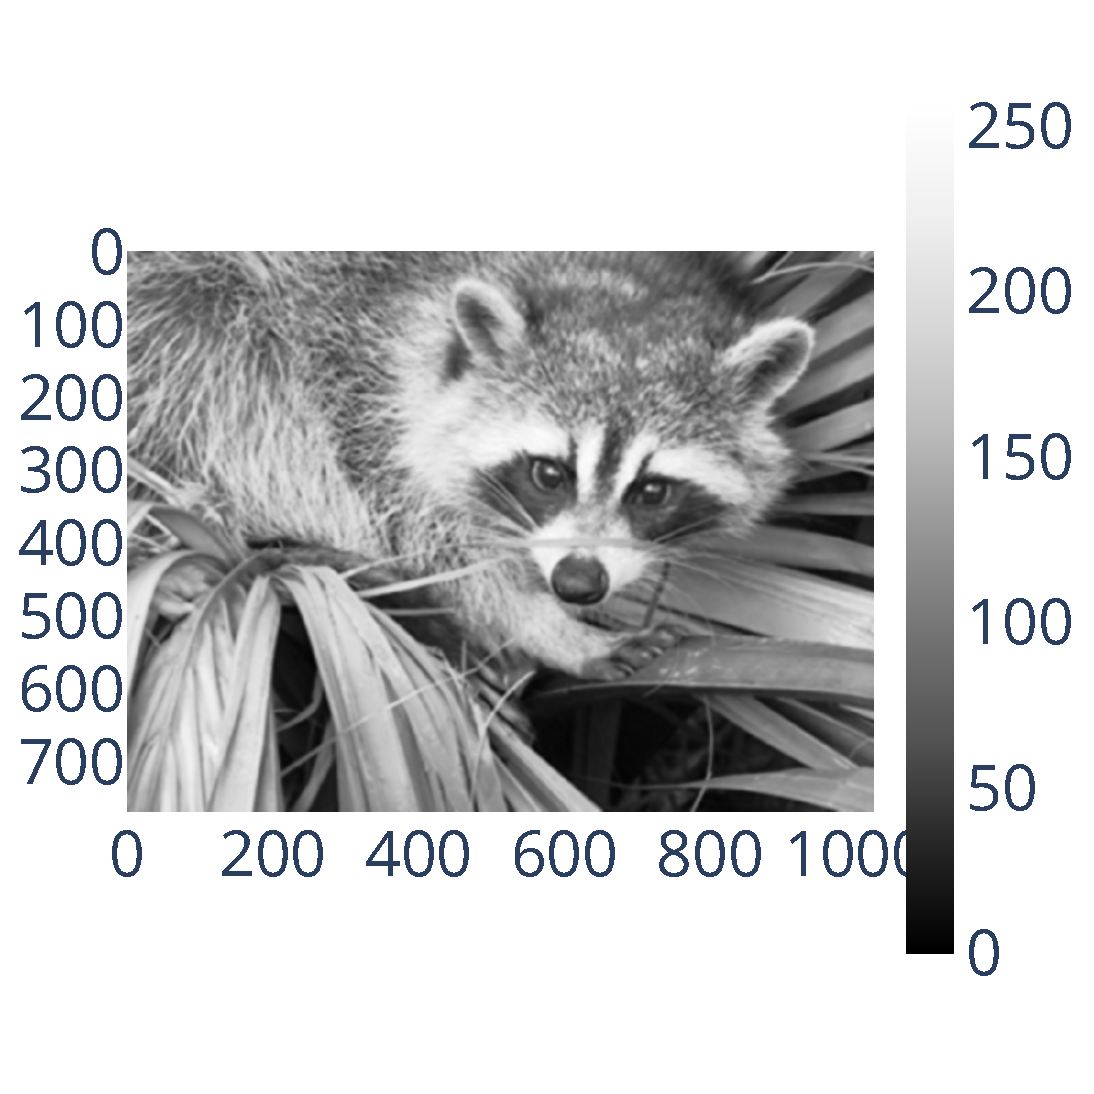
\includegraphics[width=\linewidth]{figure/bspline/original_image.pdf}
        \caption{Original image.}
        \label{fig:bspline_original_image}
    \end{subfigure}\\
    \begin{subfigure}{0.3\linewidth}
        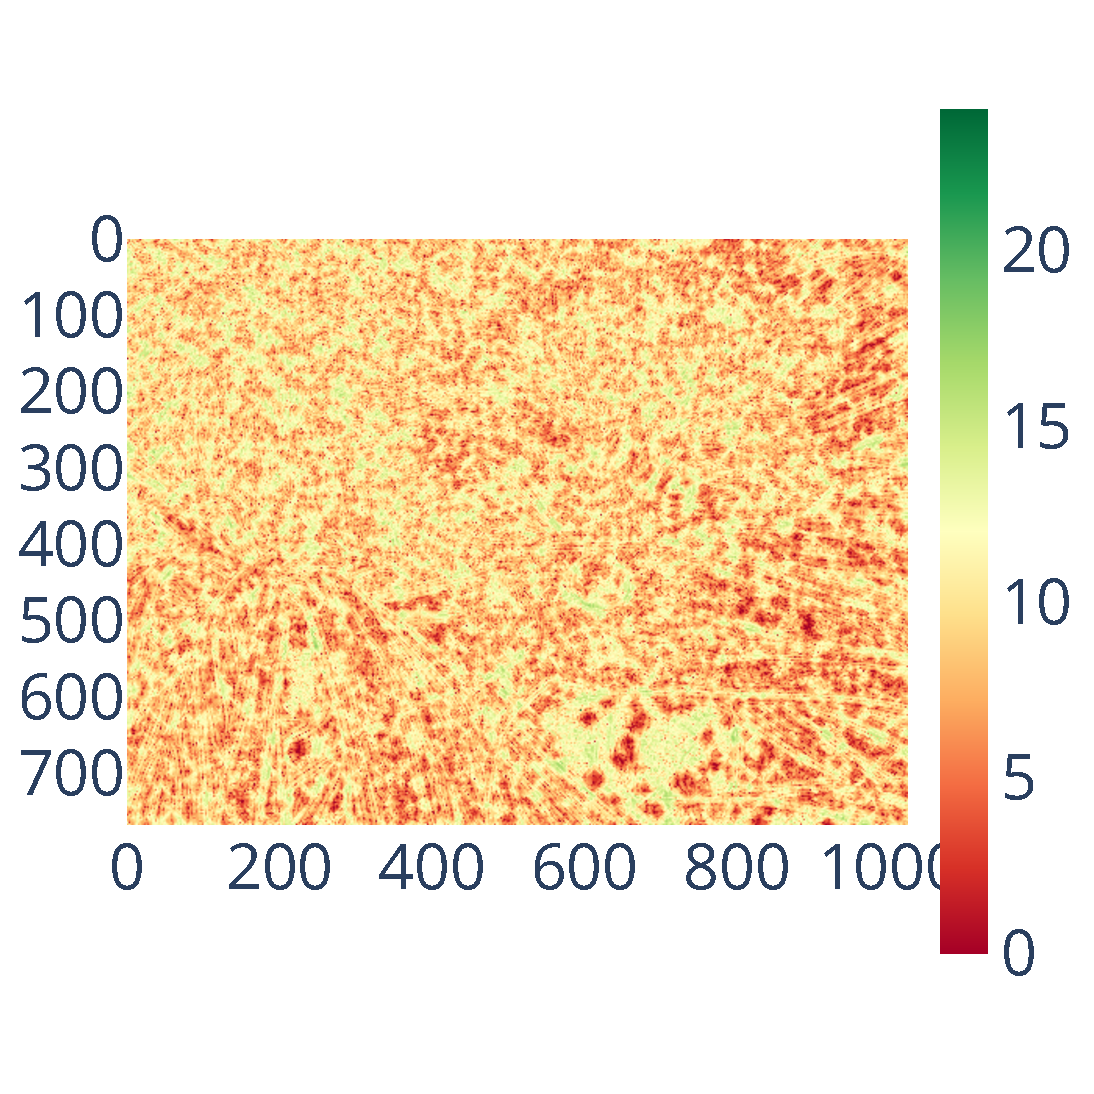
\includegraphics[width=\linewidth]{figure/bspline/bspline_sig.pdf}
        \caption{\centering\texttt{sepfir2d} significant bits}
        \label{fig:bspline_bisplev_sig}
    \end{subfigure}
    \begin{subfigure}{0.3\linewidth}
        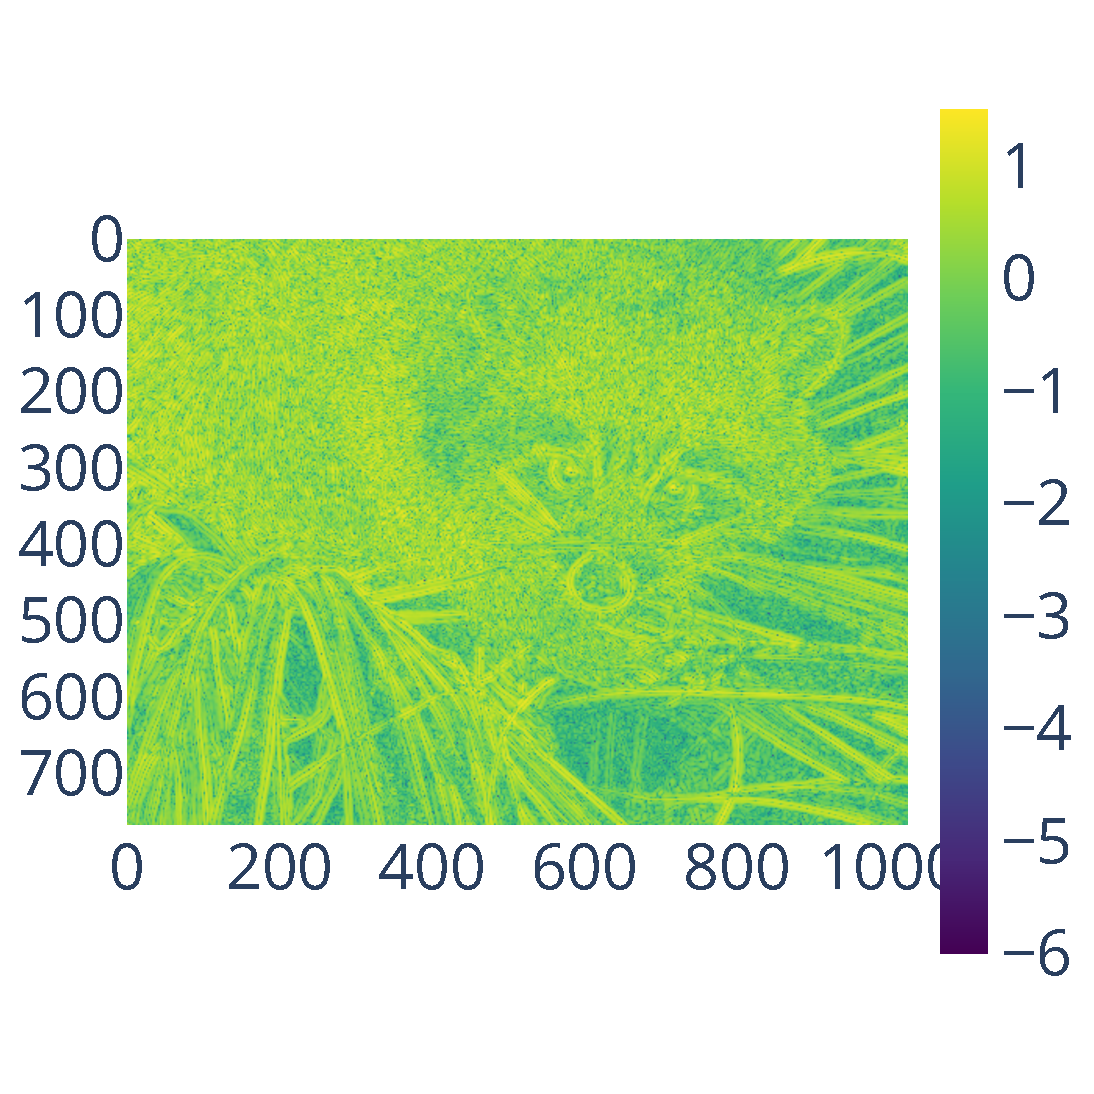
\includegraphics[width=\linewidth]{figure/bspline/bspline_mean_log.pdf}
        \caption{\centering\texttt{sepfir2d} mean (log)}
        \label{fig:bspline_bisplev_mean}
    \end{subfigure}
    \begin{subfigure}{0.3\linewidth}
        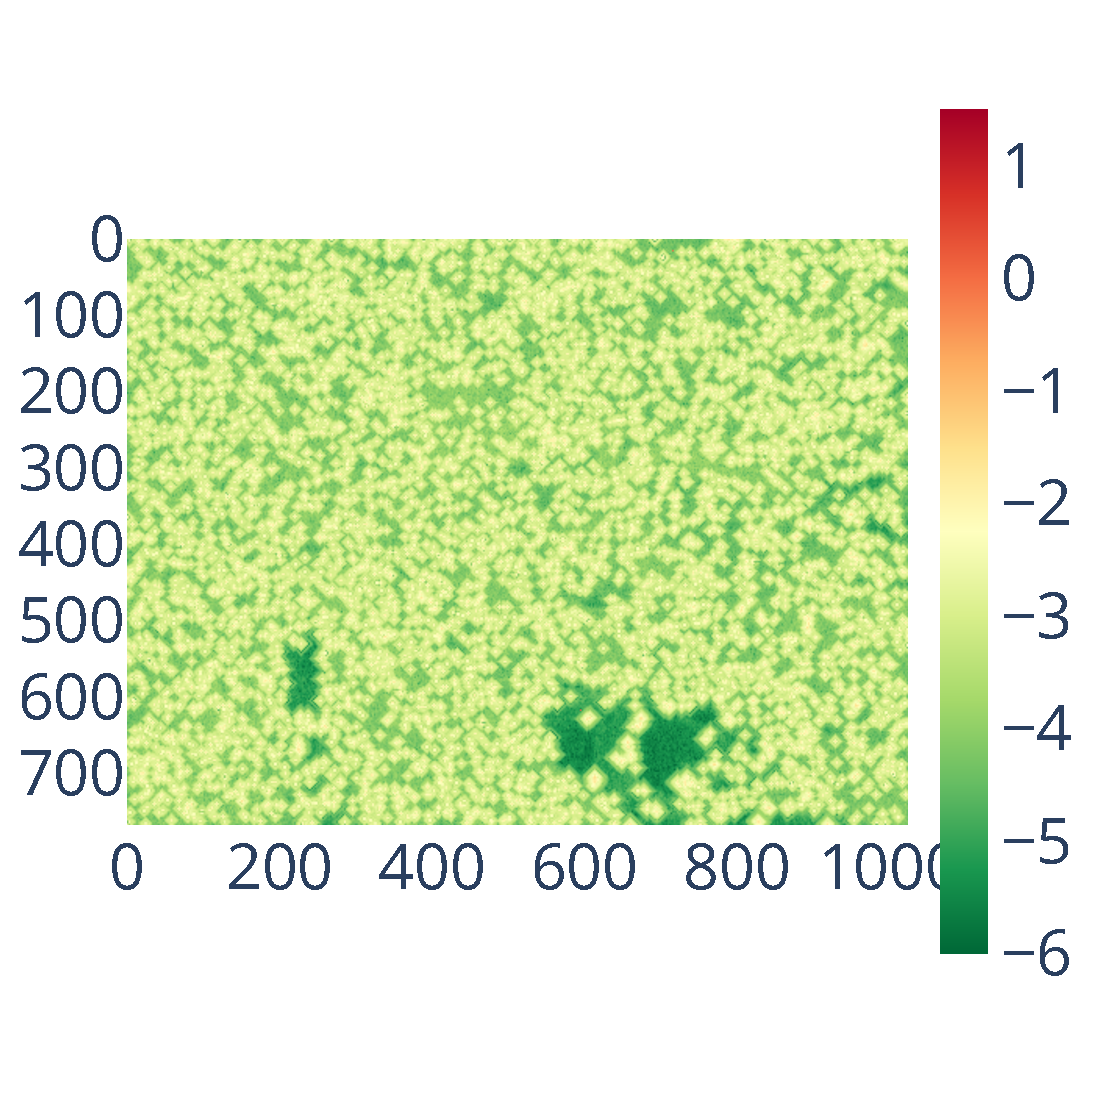
\includegraphics[width=\linewidth]{figure/bspline/bspline_std_log.pdf}
        \caption{\centering\texttt{sepfir2d} standard deviation (log)}
        \label{fig:bspline_bisplev_std}
    \end{subfigure}
    \begin{subfigure}{0.3\linewidth}
        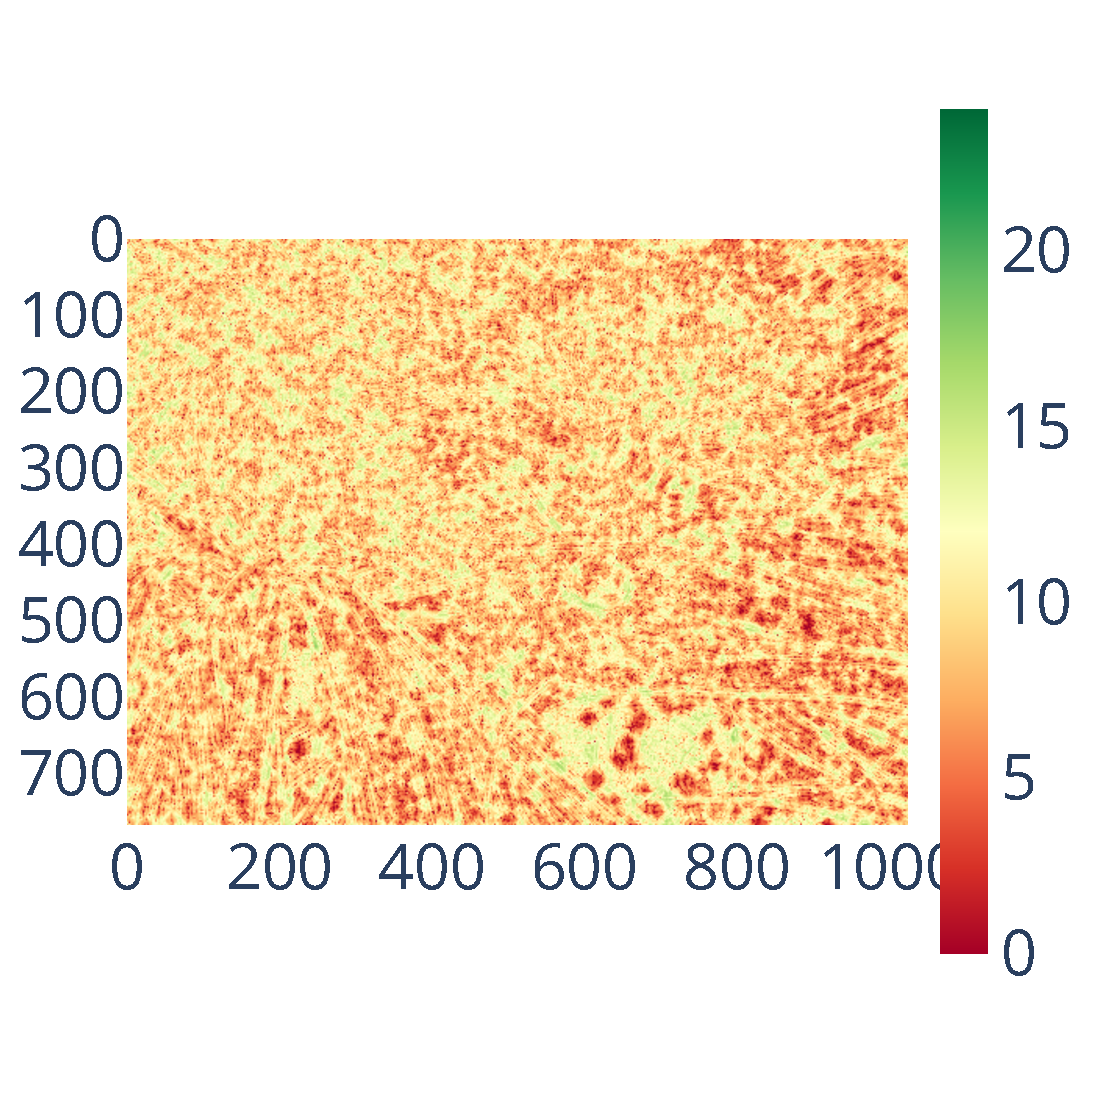
\includegraphics[width=\linewidth]{figure/bspline/convol2d_sig.pdf}
        \caption{\centering\texttt{convol2d} significant bits}
        \label{fig:bspline_convol2d_sig}
    \end{subfigure}
    \begin{subfigure}{0.3\linewidth}
        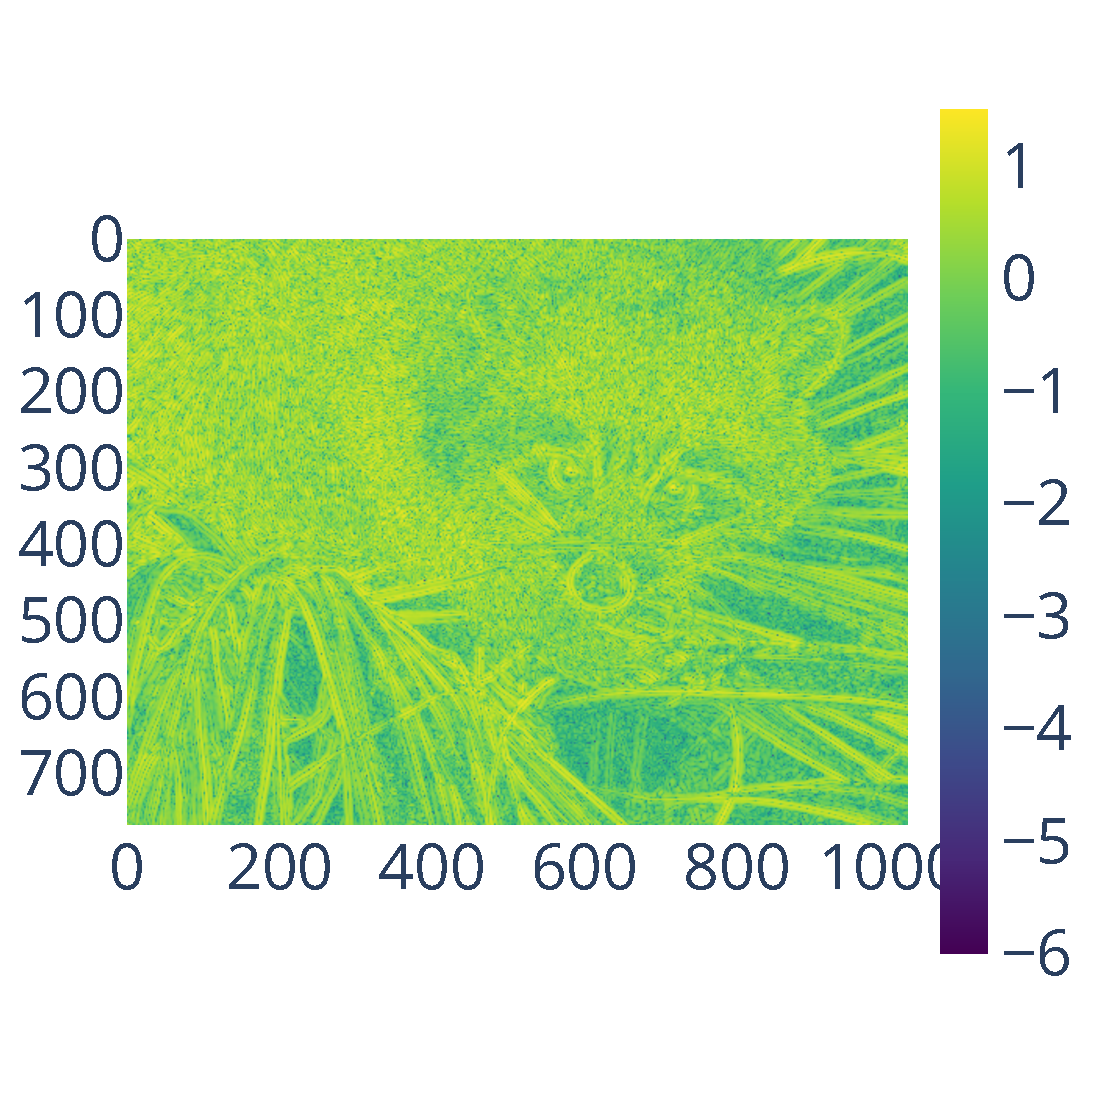
\includegraphics[width=\linewidth]{figure/bspline/convol2d_mean_log.pdf}
        \caption{\centering\texttt{convol2d} mean (log)}
        \label{fig:bspline_convol2d_mean}
    \end{subfigure}
    \begin{subfigure}{0.3\linewidth}
        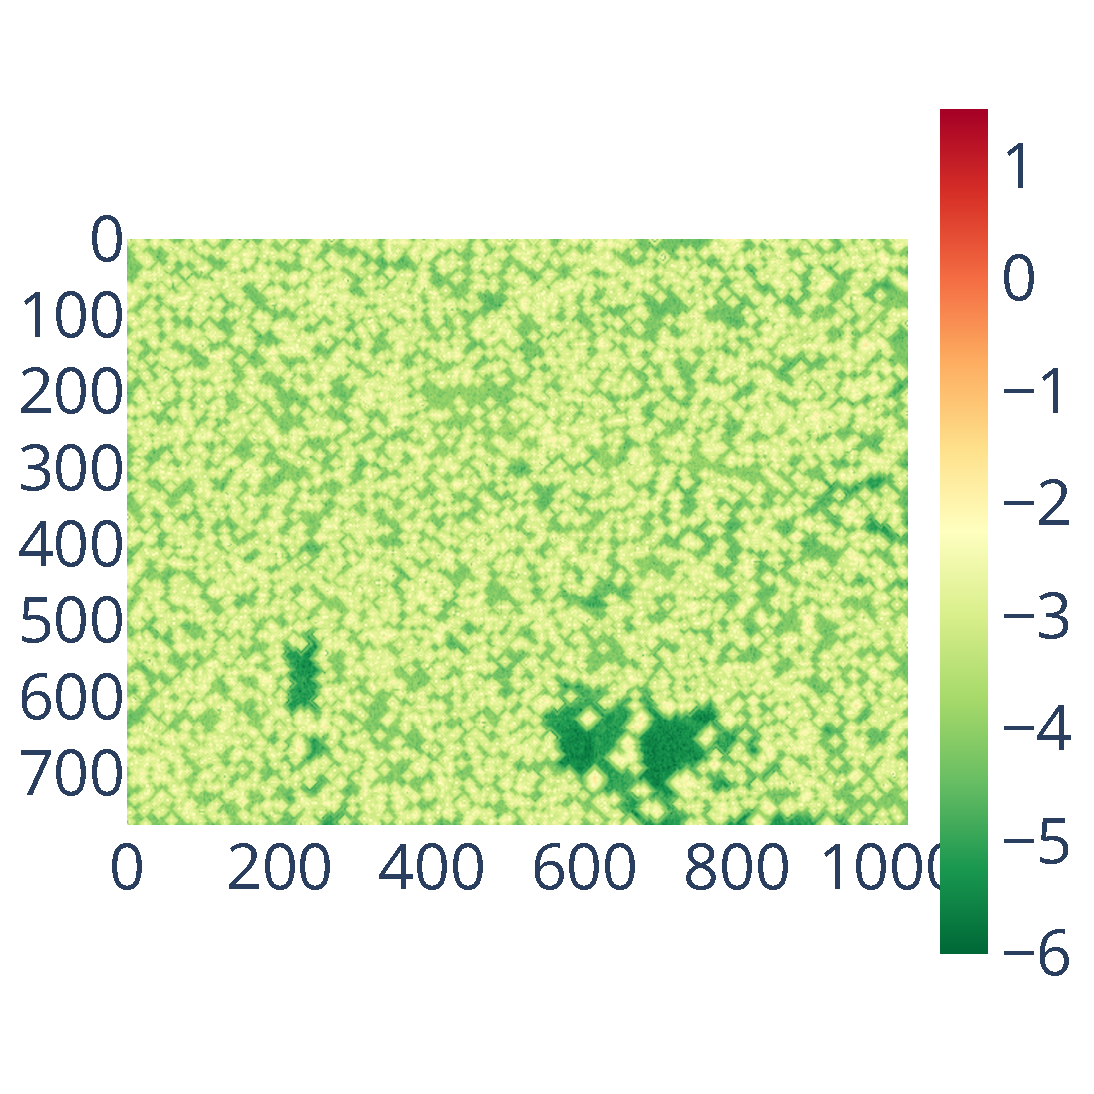
\includegraphics[width=\linewidth]{figure/bspline/convol2d_std_log.pdf}
        \caption{\centering\texttt{convol2d} standard deviation (log)}
        \label{fig:bspline_convol2d_std}
    \end{subfigure}
    \caption{\texttt{bspline} results within RR mode. \texttt{sepfir2d} and
        \texttt{convol2d} have a similar precision.
    }
    \label{fig:bspline_rr}
\end{figure}

\subsection{FFT}

This package has three examples : \texttt{discrete\_cosine\_transform},
\texttt{fft\_1D}, and \texttt{fft\_2D}. All computations are done in double
precision. The results for \texttt{discrete\_cosine\_transform},\texttt{fft\_1D}
and  \texttt{fft\_2D} show precise numerical results with 48 significant bits on
average. We observe that the FFT computation is stable to noisy inputs.
Figures~\ref{fig:fft1D_inputs} (inputs) and~\ref{fig:fft1D_outputs} (outputs)
show the mean and standard deviation of the MCA samples. The three columns
correspond to the FFT computations of:
\begin{enumerate}
    \item $z_1 = \sin(50 . 2\pi . x_i) + \dfrac{1}{2} \sin(80 . 2\pi . x_i),\; x_i = \frac{i}{600},\; i \in [0,600]$
    \item $\mathrm{blackman}(400) \times z_1$
    \item $ z_2= e^{50 . i 2\pi . x_i} + \dfrac{1}{2} e^{-80 . i2\pi .x_i },\; x_i = \frac{i}{800},\; i \in [0,400] $
\end{enumerate}

\add{The} top row in Figures~\ref{fig:fft1D_inputs} and~\ref{fig:fft1D_outputs} show the
input mean value while the bottom row shows the standard deviation. The points
with low magnitude in Figure~\ref{fig:fft1D_inputs} correspond to inputs near 0
when the input of $\sin$ or $\exp$ is close to $k\pi$, $k \in \mathbb{Z}$.
Indeed, since MCA introduces a slight noise, the result is not exactly 0. We can
see in Figure~\ref{fig:fft1D_inputs} that the maximal noise introduced by MCA on
the inputs is in the order of $10^{-14}$, two orders of magnitude higher than
the $ulp \simeq 10^-16$ for double precision. This slight noise introduced can
be interpreted as white noise on the input signal. We can see on the bottom row
of Figure~\ref{fig:fft1D_outputs} that the frequency noise is of the same order
of of magnitude as the input noise, which is expected. The two peaks at x=38 and
x=562 corresponds to the actual frequencies of the input signal.

\subsection{Optimization}

This package has eleven examples. Seven examples involve the same optimization
problem solved with and without constraints using different methods. One example
optimizes a chemical problem under constraints. The last three examples solve a
different problem each.

\subsubsection{Unconstrained minimization of multivariate scalar functions}
Four Quasi-Newton-Raphson methods minimize function $f$ by using Newton's step:
$x_{k+1} = x_{k} - B^{-1}(x_k)\nabla f(x_k)$, where $\nabla$ and $B$ are the
gradient and the approximation of the Hessian matrix of $f$. The
\texttt{Broyden-Fletcher-Goldfarb-Shanno}~\cite{BFGS} (BFGS) and
\texttt{Newton-Conjugate-Gradient}~\cite{nocedal2006numerical} (NCG) are line
search methods that approximate $H$ by adding two symmetric rank-one matrices
and by using the Conjugate-Gradient method. The \texttt{Trust-Region Truncated
    Generalized Lanczos / Conjugate Gradient}~\cite{gould1999solving} (TR-Krylov),
\texttt{Trust-Region Newton-Conjugate-Gradient} (TR-NCG), and
\texttt{Trust-Region Nearly Exact}~\cite{nocedal2006numerical} (TR-Exact) are
trust-region methods approximating $H$ by solving the trust-region subproblem
restricted to a truncated Krylov subspace and by solving nonlinear equations for
each quadratic subproblem. In addition, the
\texttt{Nelder-Mead}~\cite{singer2009nelder} simplex-based method iteratively
transforms a simplex until its vertices are getting closer to a local minima of
the function. All methods are applied to the Rosenbrock function.

\paragraph{Constrained minimization of multivariate scalar functions}
Two optimizers solve an optimization problem by taking into account constraints.
The \texttt{Sequential Least SQuares Programming} uses the
SLSQP~\cite{kraft1988software} method to optimize the Rosenbrock function. The
\texttt{Least-squares minimization} uses the Trust Region Reflective
algorithm~\cite{li1993centering} to solve a fitting problem from an enzymatic
reaction.

The SLSQP and unconstrained minimization methods minimize the
\textbf{Rosenbrock} function of $N$ variables that reaches its minimum (0) when
$x_i=1,\; \forall i \leq N-1$:
$f(x) = \sum_{i=1}^{N-1} 100(x_{i+1}-x^2_i)^2 + (1-x_i)^2$.
Figure~\ref{fig:unconstrained_optimization} shows the number of significant bits
of the solution for the different methods used. The $(p)$ notation for the NCG,
Trust-Krylov, and Trust-NCG methods in the legend refers to the variant where
the Hessian matrix is replaced by a function computing the matrix-vector product
of the Hessian and an arbitrary vector, to save memory and time. All the methods
have a good precision ranging from 43 to 53 significant bits. The Nelder-Mead
method is the least precise one with $\simeq$ 43 significant bits on average,
while the Trust-Region-Newton-CG is the most precise one with $\simeq$ 53
significant bits, the highest precision achievable in double precision. The
remaining methods have a similar precision.

The SLSQP also minimizes the Rosenbrock function with the following constraint:
$x_0$ + $2x_1$ $\leq$ 1
$x_0^2$ + $x_1$ $\leq$ 1
$x_0^2$ - $x_1$ $\leq$ 1
$2x_0$ + $x_1$ = 1
0 $\leq$ $x_0$ $\leq$ 1
-0.5 $\leq$ $x_1$ $\leq$ 2.
% \begin{eqnarray*}
%     x_0 + 2x_1 \leq 1 \\
%     x_0^2 + x_1 \leq 1 \\
%     x_0^2 - x_1 \leq 1 \\
%     2x_0 + x_1 = 1 \\
%     0 \leq x_0 \leq 1 \\
%     -0.5 \leq x_1 \leq 2 
% \end{eqnarray*}
The problem has a unique solution $[x_0, x_1] = [0.4149, 0.1701]$. Results
obtained with RR show a precision of 47 and 44 significant bits for the first
and the second solution. %\tristan{which method is tested?}.

The \texttt{least-square minimization} example solves a fitting problem from an enzymatic reaction~\cite{kowalik1968analysis} with 11 residuals defined as:
\begin{eqnarray*}
    f_i(x) &=& \frac{x_0(u_i^2 + u_ix_1)}{u_i^2 + u_ix_2+x_3}-y_i,\; i=0,...,10 \\
    &0& \leq x_j \leq 100,\; j=0,..,3
\end{eqnarray*}
where where $y_i$ are measurement values, $u_i$ are values of the independent
variable, and $x_i$ the unknown. Results within RR show a precision of 51, 46,
47, and 48 significant bits for each component of the solution
respectively.% \tristan{which solver is used?}.

\subsubsection{Root finding}
% We tested three root finder algorithms with one for small problems using the hybrid Powell and Levenberg-Marquardt methods  (\texttt{root\_finding}) and two for large problems using a Krylov approximation for the inverse Jacobian with and without the help of a preconditioner (\texttt{root\_finding\_large\_preconditionned} and \texttt{root\_finding\_large}).

The \texttt{root\_*} examples use three algorithms to find the root of
non-linear equations. \texttt{root\_finding} uses the hybrid Powell method to
solve a single-variable transcendental equation and the Levenberg-Marquardt
method for a set of non-linear equations. \texttt{root\_finding\_large} and
\texttt{root\_finding\_large\_preconditioned} examples use the Krylov method to
approximate the inverse Jac\add{o}bian with and without the help of a preconditioner.
They solve an integrodifferential equation on a square $(x,y) \in [0,1] \times
    [0,1]$, $P(x,1)=1$, and $P=0$ elsewhere on the boundary. The function $P$ is
discretized with a Cartesian grid $P_{n,n}=P(nh,nh)$, with $n=75$, and its
derivatives are approximated by $\partial_x^2P(x,y) \simeq (P(x+h,y) - 2P(x,y) +
    P(x-h,y))/h^2$.

% the two following equations: $x + 2\cos(x) = 0$ and 
% the set $x_0\cos(x_1)=4$; $x_0x_1-x_1 = 5$ while the 
% \texttt{root\_finding\_large} and \texttt{root\_finding\_large\_preconditioned} tests 
% solve the equation:
% \[
%     (\partial_x^2 + \partial_y^2)P + 5 \left(\int_0^1 \int_0^1 cosh(P)\, dx dy \right)^2 = 0
% \]

All the examples diverge even within RR, which is not surprising since
root-finding methods can easily take a few extra steps to find the root
depending on the starting point. Nevertheless, for the
\texttt{root\_finding\_large} example, 3 traces among the 5 samples can be
merged for both RR and MCA modes. Figure~\ref{fig:root_finding_large} shows the
mean and standard deviation of the result for these 3 samples. We can see that a
similar solution was found for RR and Full MCA. Full MCA leads to a lower
precision than RR although both standard deviation maps remain in the same order
of magnitude. Finally, it is interesting to note the impact of preconditioning
on the result numerical quality: as Table~\ref{tab:pytracer_results_summary}
shows, the precision doubles between \texttt{root\_finding\_large} and
\texttt{root\_finding\_large\_preconditioned}.

\begin{figure}
    \centering
    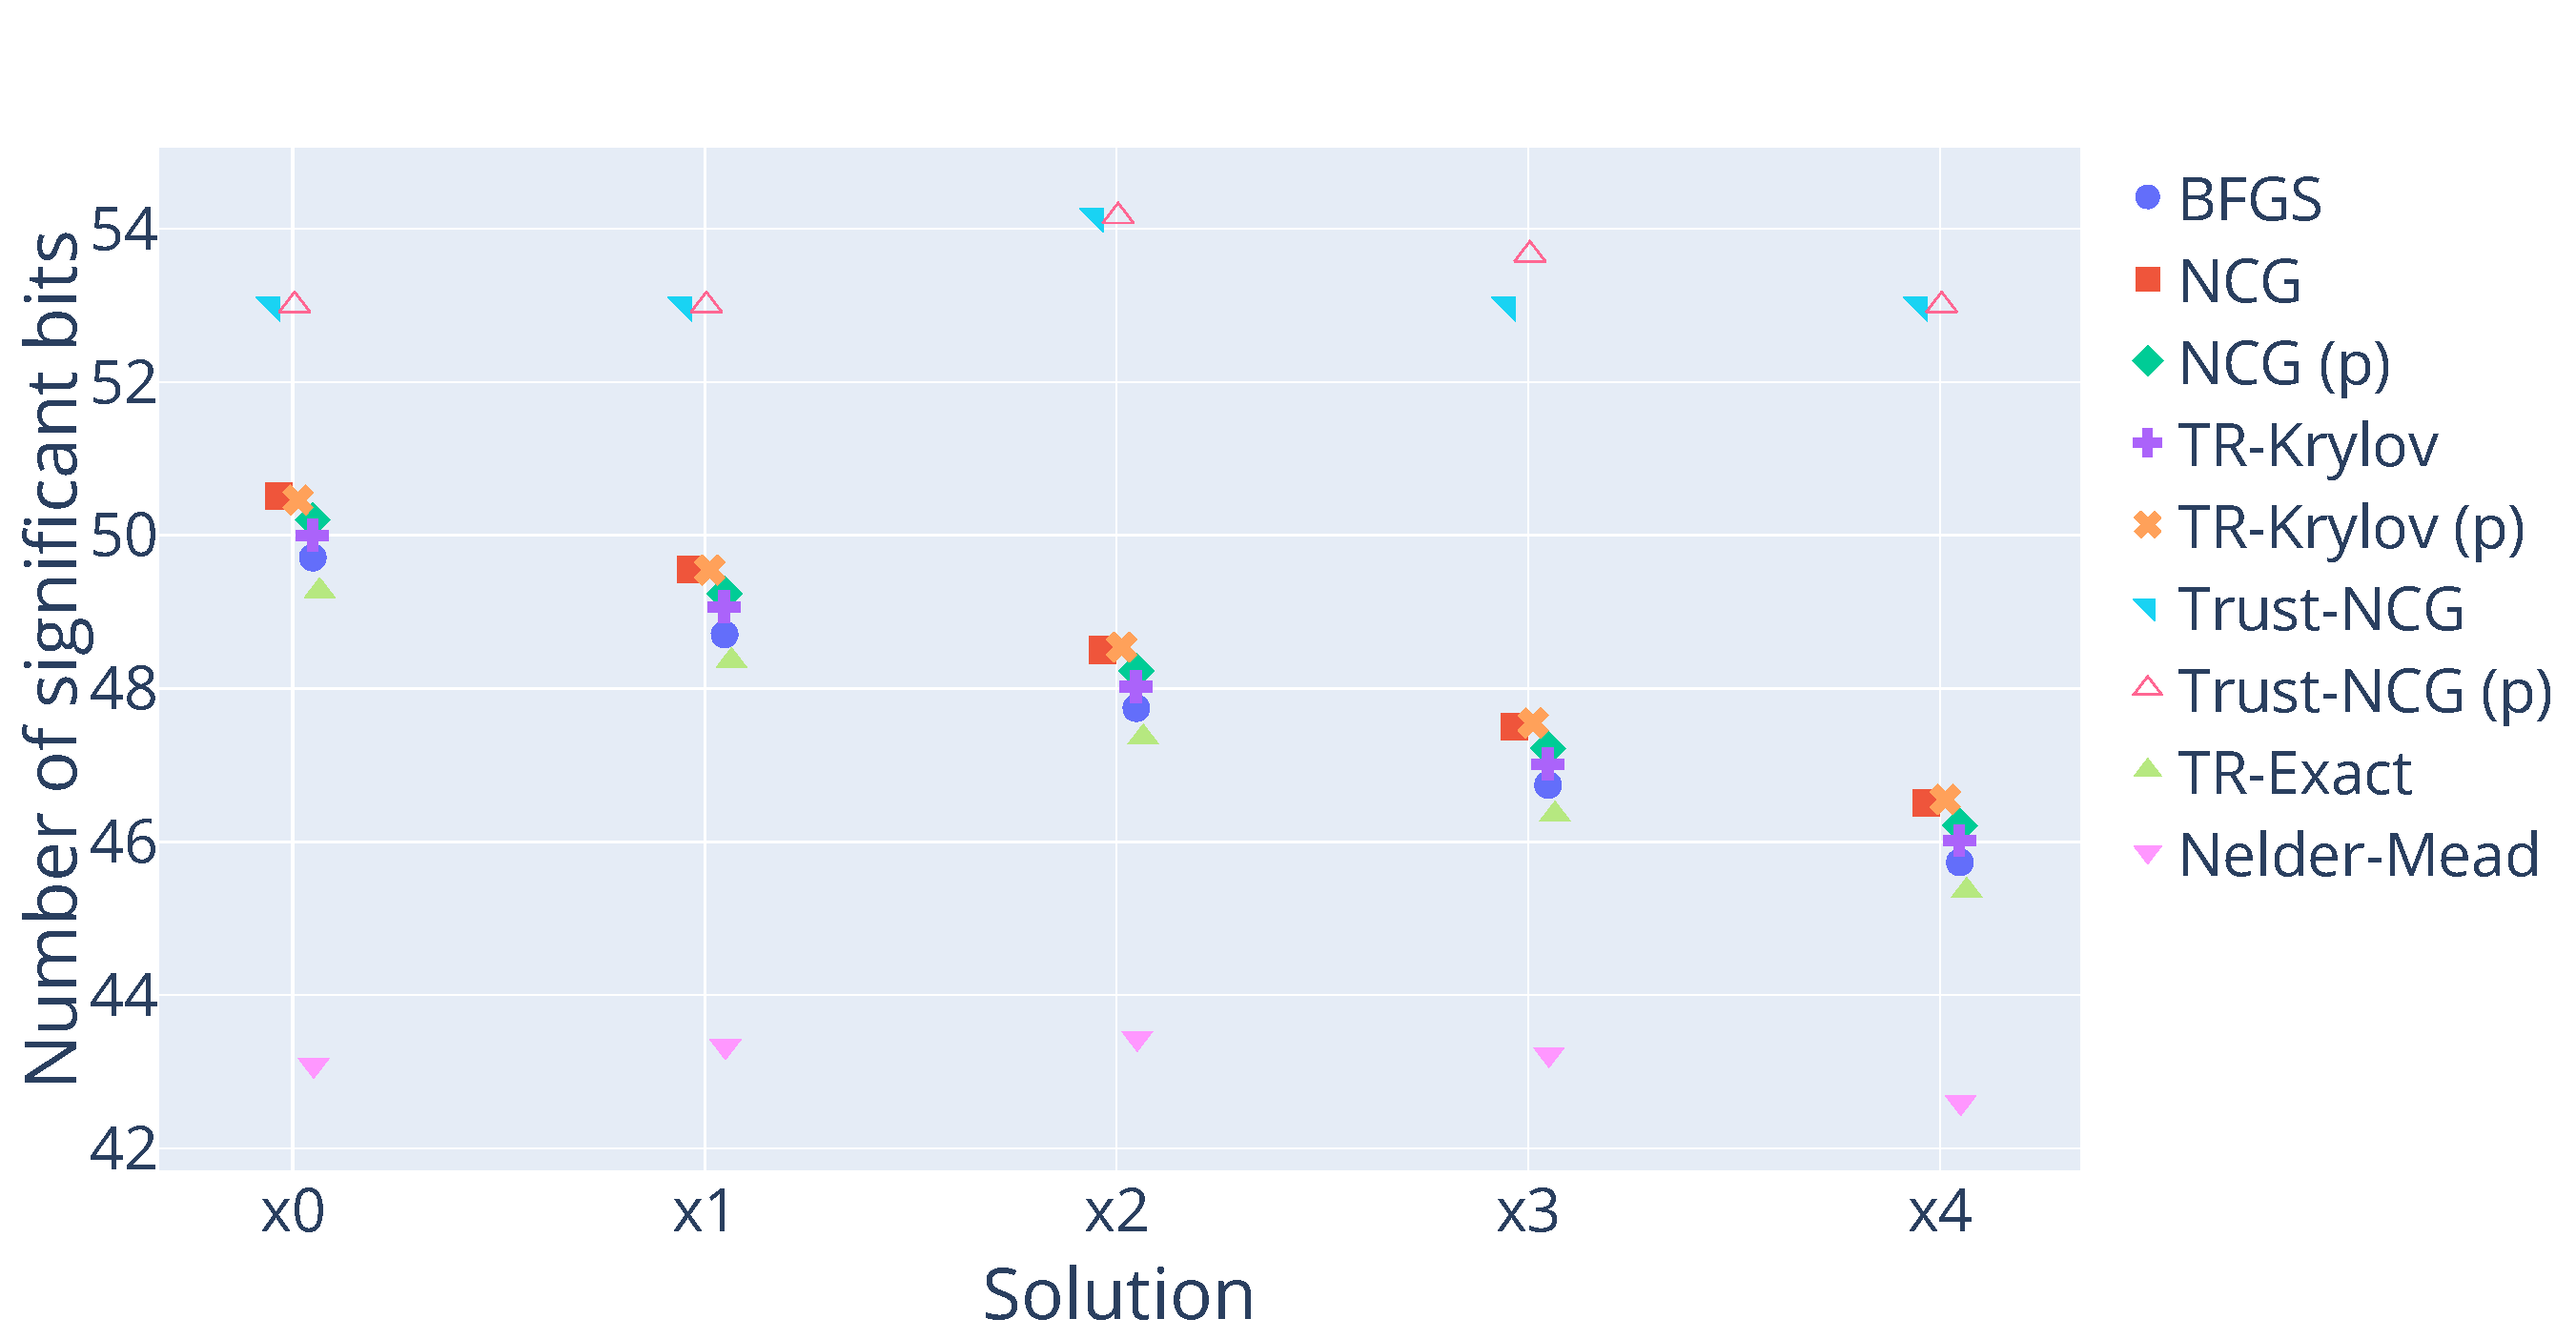
\includegraphics[width=\linewidth]{figure/unconstrained_optimization_comparison.pdf}
    \caption{Comparison of results precision for different optimization solvers within RR mode.}
    \label{fig:unconstrained_optimization}
\end{figure}

\begin{figure}
    \centering
    \begin{subfigure}{0.45\linewidth}
        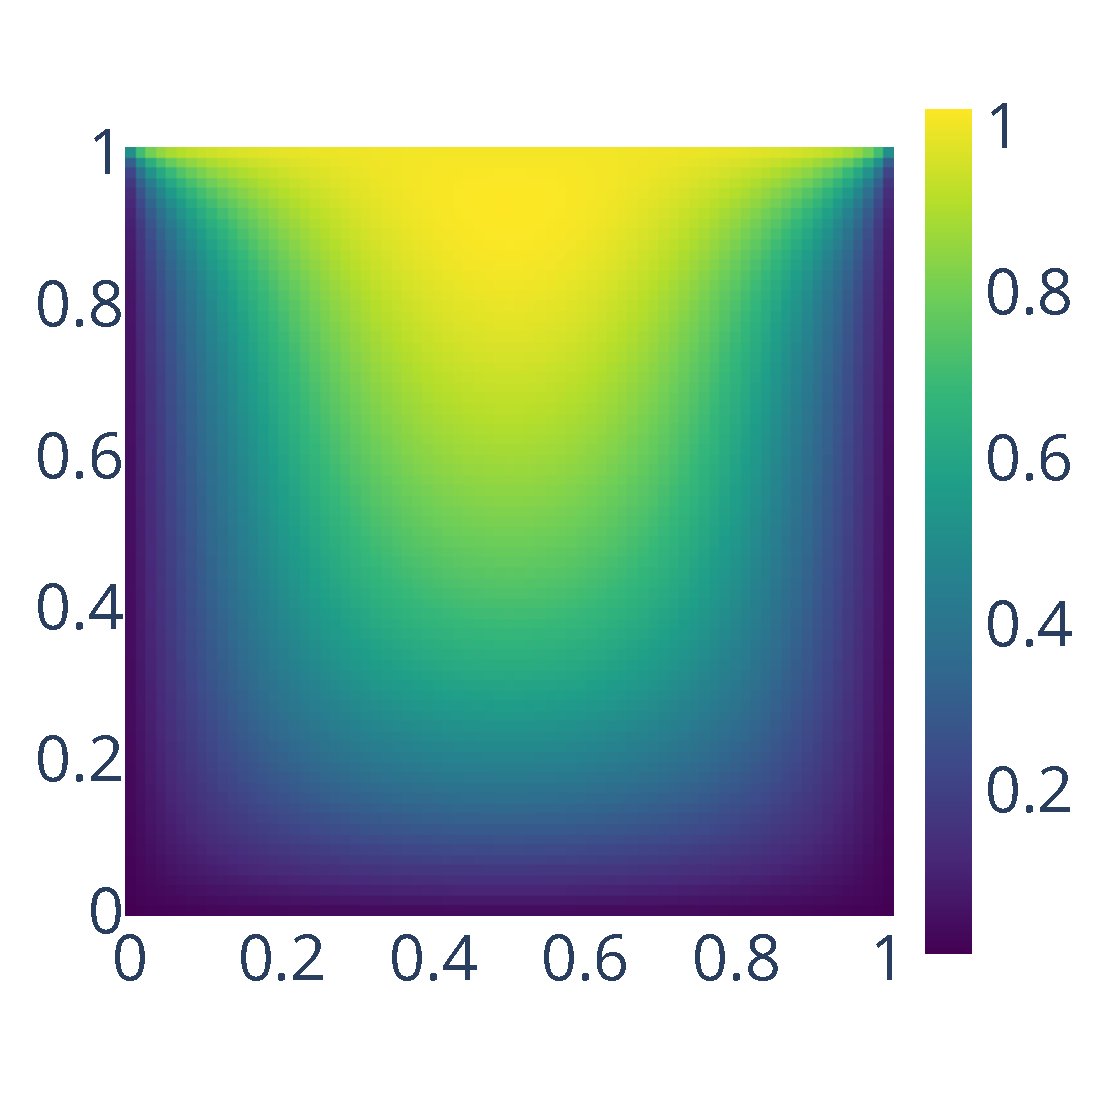
\includegraphics[width=\linewidth]{figure/root_finding/solution_mean_RR.pdf}
        \caption{Mean solution (RR)}
        \label{fig:mean_solution_rr}
    \end{subfigure}
    \begin{subfigure}{0.45\linewidth}
        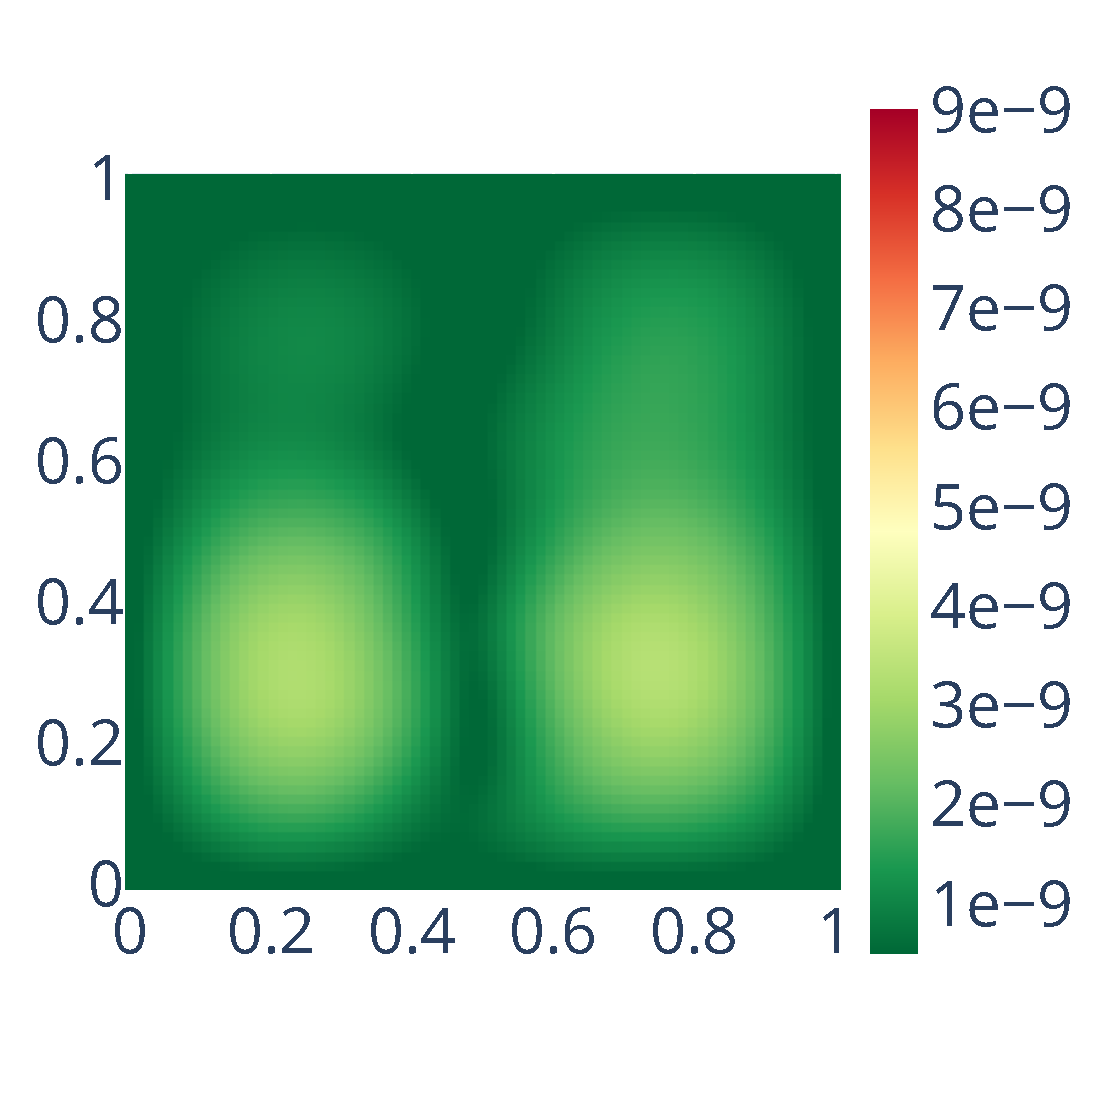
\includegraphics[width=\linewidth]{figure/root_finding/solution_std_RR.pdf}
        \caption{Standard deviation solution (RR)}
        \label{fig:stdev_rr}
    \end{subfigure}

    \begin{subfigure}{0.45\linewidth}
        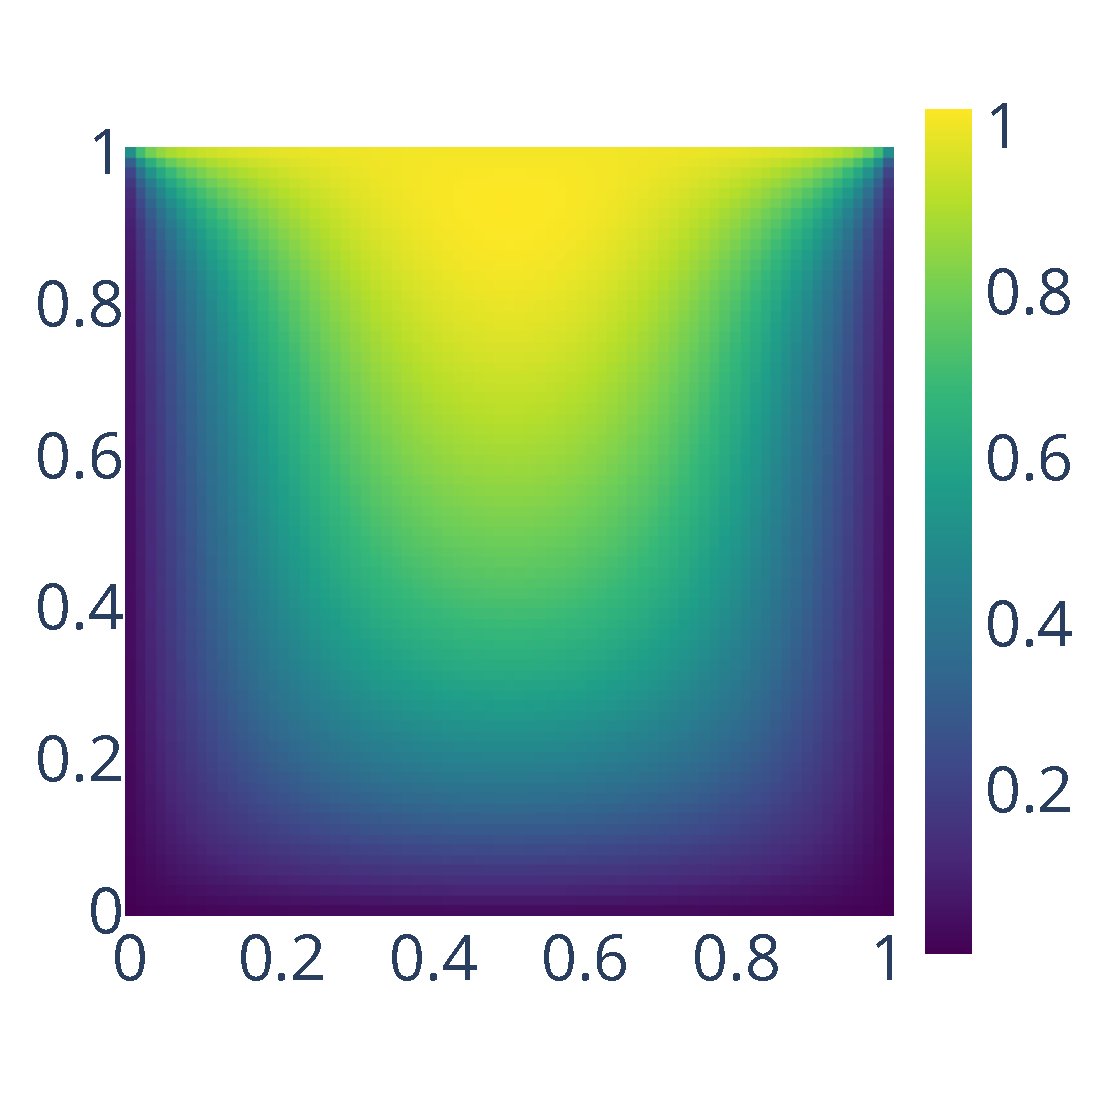
\includegraphics[width=\linewidth]{figure/root_finding/solution_mean_MCA.pdf}
        \caption{Mean solution (Full MCA)}
        \label{fig:mean_solution_mca}
    \end{subfigure}
    \begin{subfigure}{0.45\linewidth}
        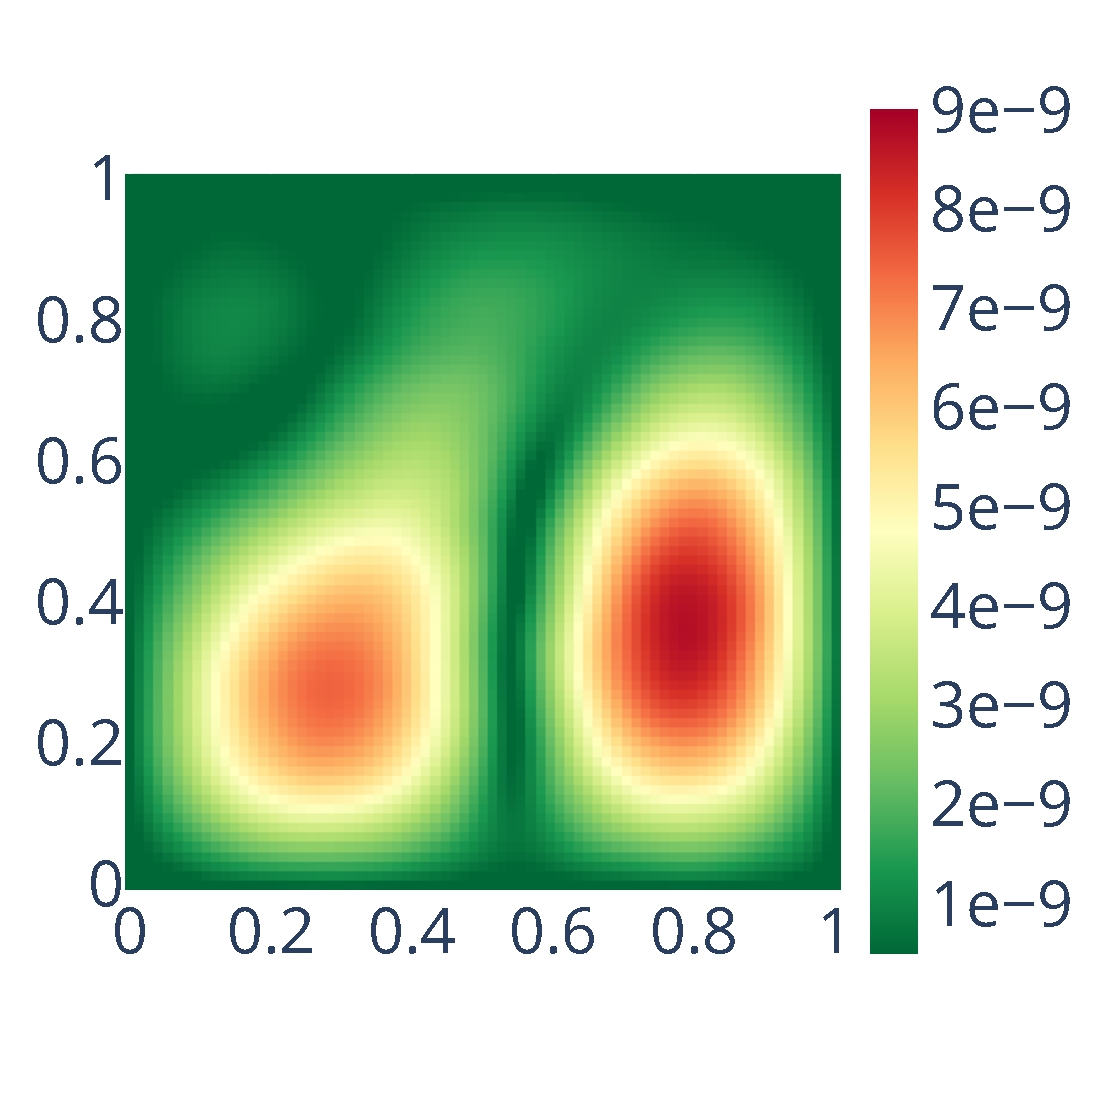
\includegraphics[width=\linewidth]{figure/root_finding/solution_std_MCA.pdf}
        \caption{Standard deviation (Full MCA)}
        \label{fig:stdev_mca}
    \end{subfigure}
    \caption{Solution of \texttt{root\_finding\_large} example.
        The standard deviation has two maximum for both RR and Full MCA modes. The standard deviation remains lower than
        the stopping criterion threshold fixed at $6.10^{-6}$. }
    \label{fig:root_finding_large}
\end{figure}

\subsection{Scikit learn}
\label{sec:sklearn_tests}

Scikit-learn offers a well-supplied and documented list of examples that
facilitates its use with Pytracer. Among the several available examples, we
choose the following representative set listed in
Table~\ref{tab:pytracer_results_summary}. The following paragraphs focus on the
most interesting stability results observed across all experiments.

\subsubsection{Separating hyperplane}

This example uses a linear Support Vector Machine (SVM) classifier trained using
the Stochastic Gradient Descent (SGD) method to find the maximum separating
hyperplane between sets of 2D points. The example trains the SVM with 50 random
points separated in 2 clusters with hyperparameter $\alpha=0.01$ and using the
hinge loss function. Once the model is trained, the example generates a
$[-1,5]\times[-1,5]$ Cartesian grid discretized with 100 points and predicts the
class label for each point with integer coordinates.
Figure~\ref{fig:hyperplan_sig_zoom} shows the number of significant bits
obtained with RR for each point of the grid.
We can see that yellow regions
close to the separating hyperplane are highly unstable with a number of
significant bits below 0, meaning that the classifier is unsure about the
predicted class.
%\tristan{Describe and comment on the other 2 tests, why are they more stable? Is it because the training set has more points?}


% \begin{figure}
%     \centering
%     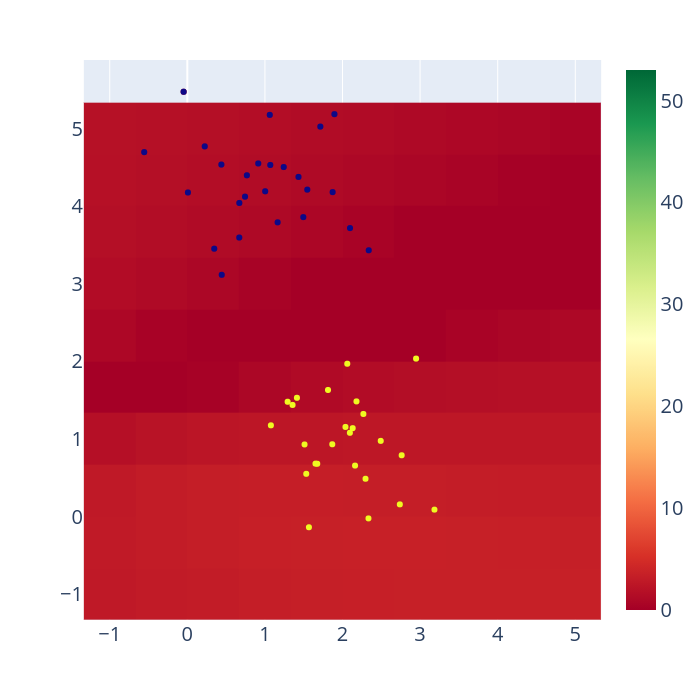
\includegraphics[width=\linewidth]{figure/separating_hyperplan/hyperplan.png}
%     \caption{Ratio $mean/std$ of Separating hyperplane test result within RR mode.
%     Circle and square points represent respectively the train and test dataset.
%     The color represents the predicted class. We can see that 
%     instability is high around the hyperplane which is coherent with 
%     the fact the classifier has difficulty to decide in which side of the hyperplane the 
%     point is.}
%     \label{fig:separating_hyperplan}
% \end{figure}

\begin{figure}
    \centering
    % \begin{subfigure}{.3\linewidth}
    % 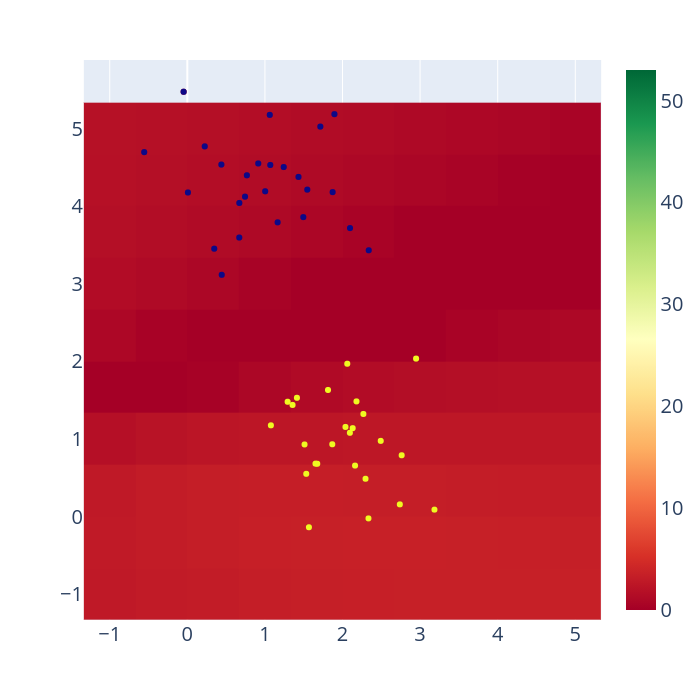
\includegraphics[width=\linewidth]{figure/separating_hyperplan/hyperplan.png}
    % \caption{}
    % \label{fig:hyperplan_sig}
    % \end{subfigure}
    \begin{subfigure}{.45\linewidth}
        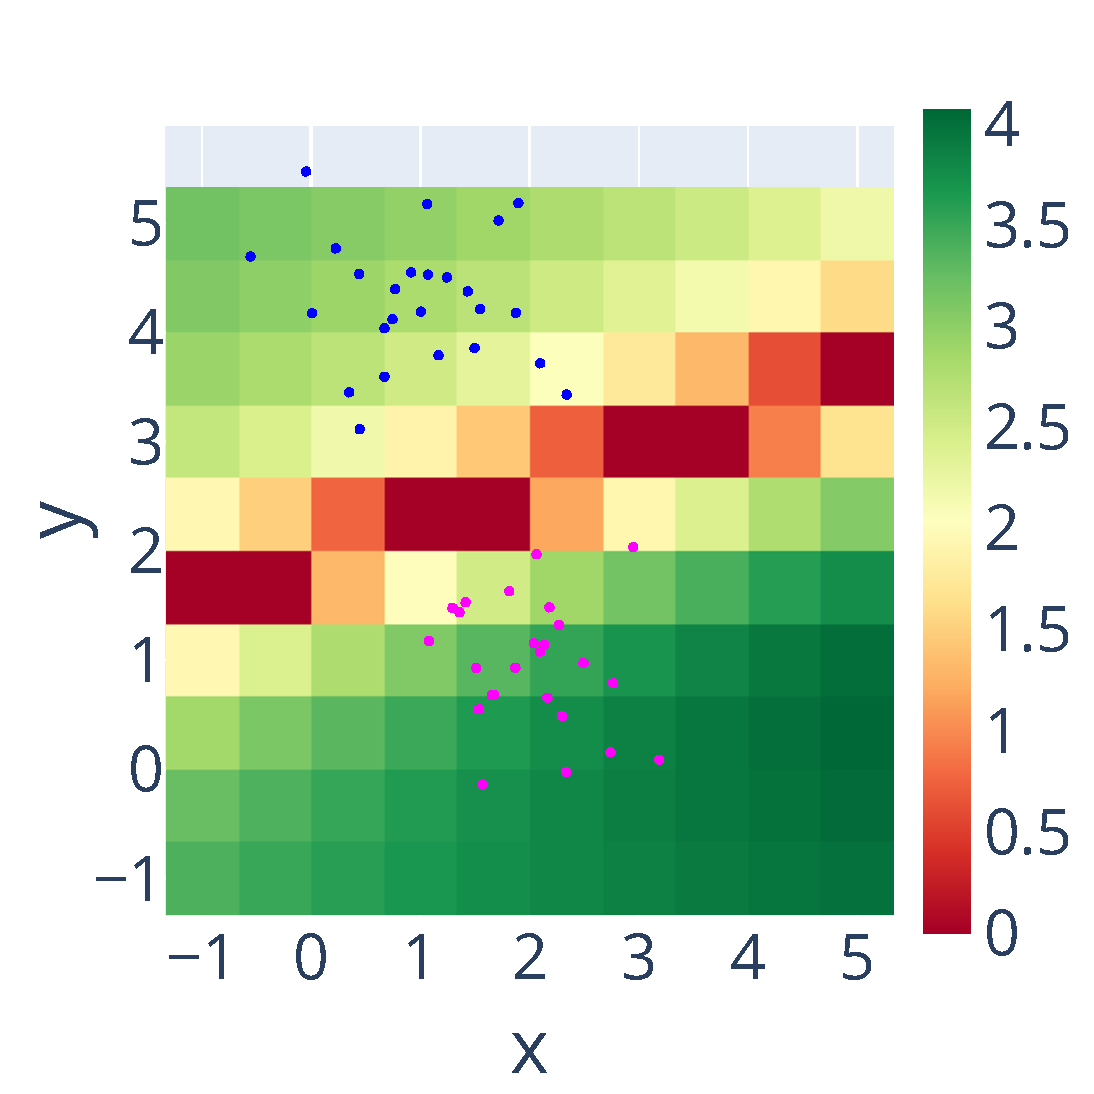
\includegraphics[width=\linewidth]{figure/separating_hyperplan/hyperplane_zoom.pdf}
        \caption{Separating hyperplane}
        \label{fig:hyperplan_sig_zoom}
    \end{subfigure} \\
    \begin{subfigure}{.45\linewidth}
        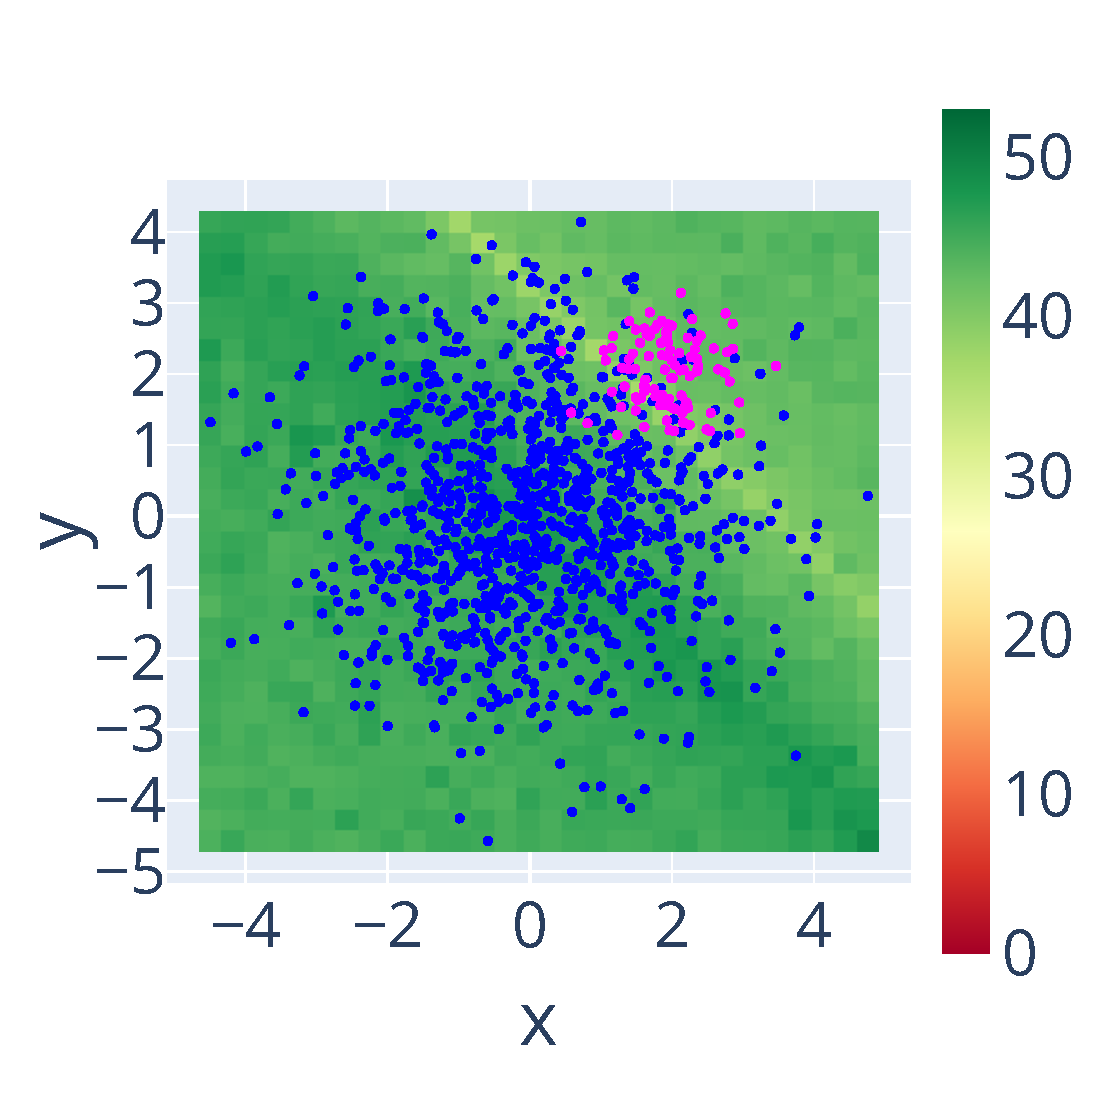
\includegraphics[width=\linewidth]{figure/SVM/non_weighted.pdf}
        \caption{SVM (non weighted)}
        \label{fig:SVM_nw_sig}
    \end{subfigure}
    \begin{subfigure}{.45\linewidth}
        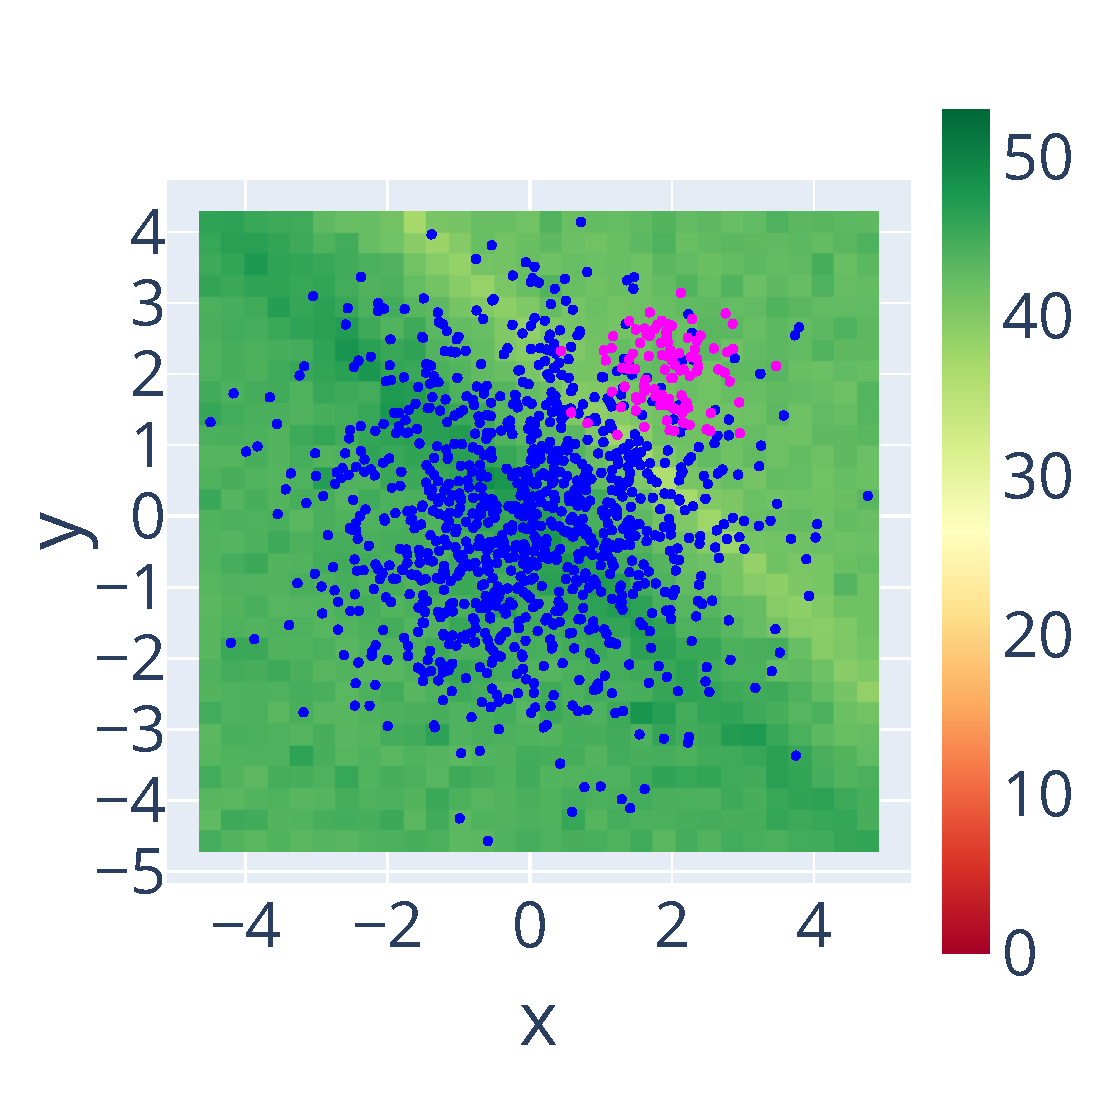
\includegraphics[width=\linewidth]{figure/SVM/weighted.pdf}
        \caption{SVM (weighted)}
        \label{fig:SVM_w_sig}
    \end{subfigure} \\
    \begin{subfigure}{.45\linewidth}
        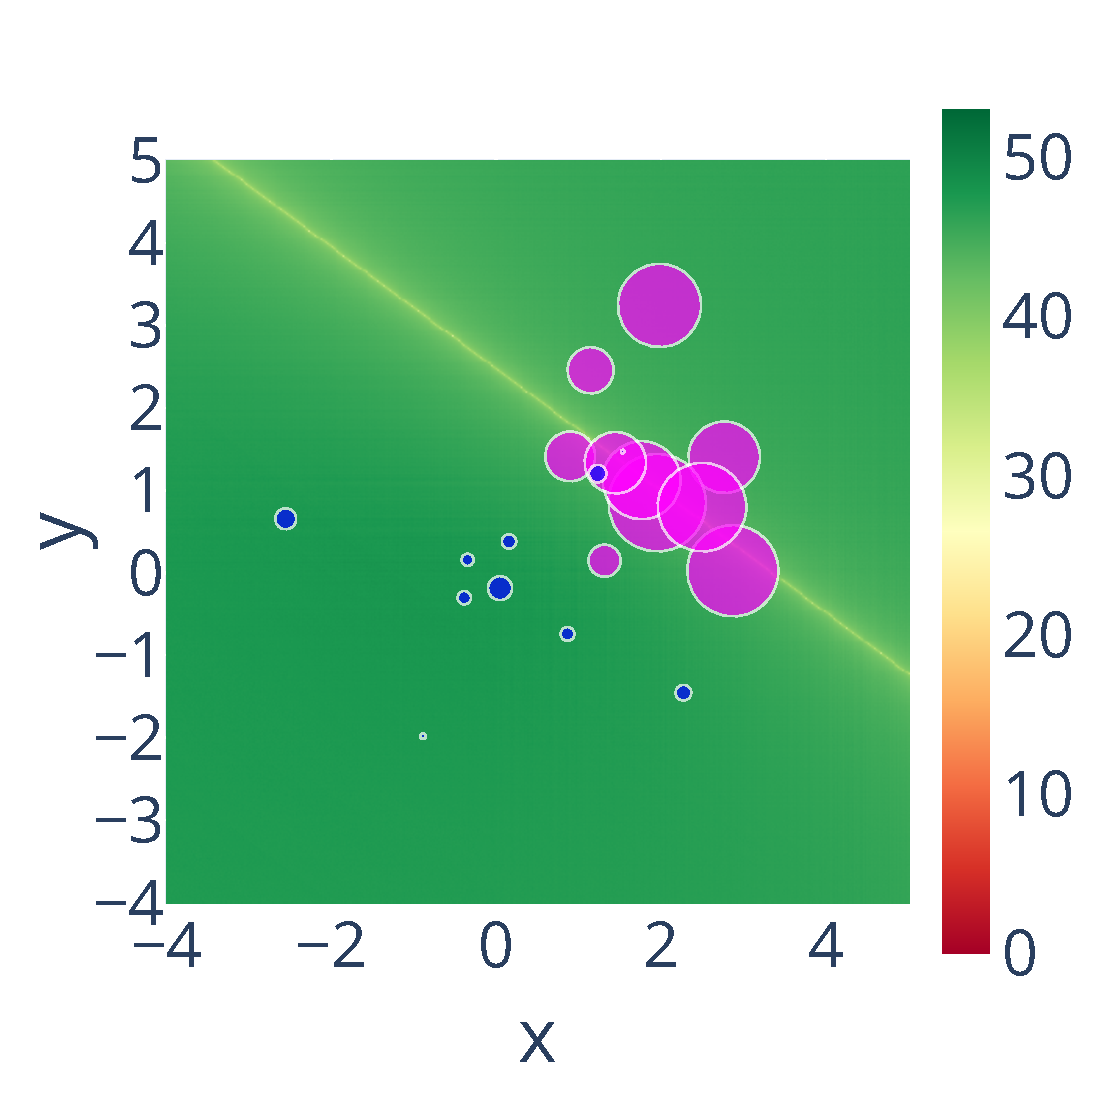
\includegraphics[width=\linewidth]{figure/Weighted/non_weighted.pdf}
        \caption{SGD weighted (non-weighted)}
        \label{fig:weighted_nw_sig}
    \end{subfigure}
    \begin{subfigure}{.45\linewidth}
        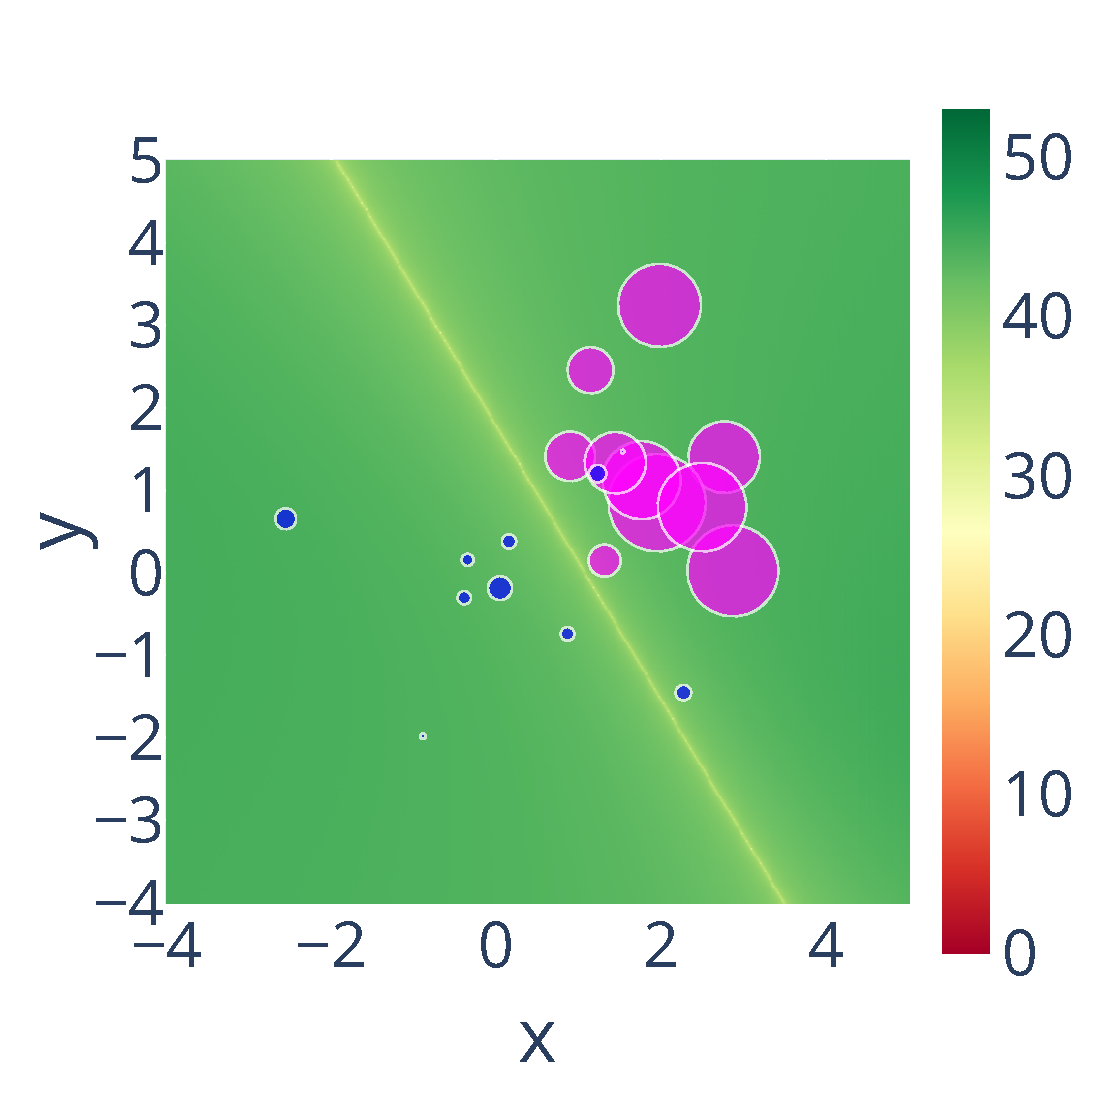
\includegraphics[width=\linewidth]{figure/Weighted/weighted.pdf}
        \caption{SGD weighted (weighted)}
        \label{fig:weighted_w_sig}
    \end{subfigure}
    \caption{
        Three examples of separating hyperplane prediction. All the figures show the number of significant bits of the prediction in RR mode. The separating hyperplane corresponds to a lower-precsion region in each figure. Using a large discretization step amplifies
        this instability.
        % respectively the results of examples    \textit{SVM} and~\textit{Weighted samples}. Figures~\ref{fig:SVM_nw_sig} and~\ref{fig:weighted_nw_sig} show the unweighted classification while Figures~\ref{fig:SVM_w_sig} and~\ref{fig:weighted_nw_sig} the classification taking into account the weights. We can see that taking into account the weight classes allows a better separation. 
        % \tristan{add labels to subfigures} \tristan{don't use this yellow for class 1, take a color that isn't in the color map. Add a legend to show the class colors.}
    }
    \label{fig:separating_hyperplan}
\end{figure}

\subsubsection{SVM}
This example uses a plain Support Vector
Classification~\cite{Platt99probabilisticoutputs} (SVC) to find the best
hyperplane separating an unbalanced dataset with two classes of 1000 and 100
points. This example tests two SVC configurations using a linear kernel with and
without a class weight parameter. The SVC predicts the class label for each
coordinate over a $[-5,5] \times [-5,5]$ grid discretized with 900 points.
Figures~\ref{fig:SVM_nw_sig} and~\ref{fig:SVM_w_sig} show the result within RR
of the classification with and without taking into account the unbalancing. We
can see that the number of significant bits is lower on the separating line and
that taking into account class imbalance allows for a better separation.

\subsubsection{SGD weighted samples}
This example uses an SGD to separate weighted points. It divides the training
set into two classes of 10 points with a bigger weight for the second class. The
SGD is trained with hyperparameters $\alpha=0.01$ and a maximum number of
iterations to 100. The prediction is made on a $[-4,5]\times[-4,5]$ grid
discretized with 250\add{,}000 points. Figures~\ref{fig:weighted_nw_sig}
and~\ref{fig:weighted_w_sig} show the number of significant bits of prediction
within RR along with dataset points in blue and \remove{violet} \add{purple}. We can see that the
separating plane corresponds to a region of lower precision, similar to the
previous examples.

% \begin{figure}
%     \centering
%     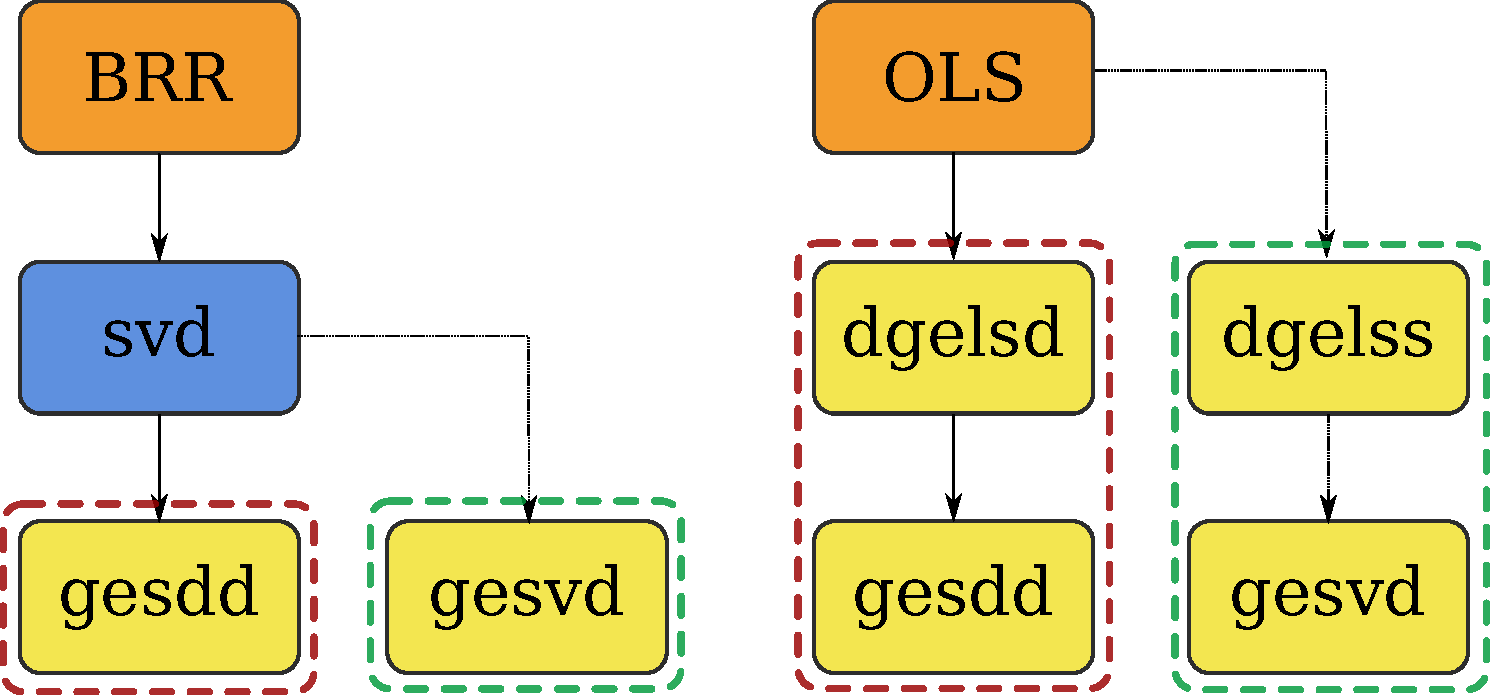
\includegraphics[width=0.5\linewidth]{figure/BRR/call_path.pdf}
%     \caption{Call paths of the Bayesian Ridge Regression (BRR) and Ordinary
%         Least Square (OLS) function. Color represents the calling library:
%         orange for scikit-learn, blue for SciPy and yellow for LAPACK. Dashed
%         color represents the original path in red and the alternative one in
%         green. Figure~\ref{fig:brr_svd_sig} shows the original method  leads to
%         numerical instabilities while the alternative one converges. }
%     \label{fig:call_path_brr}
% \end{figure}

% \begin{figure}
%     \centering
%     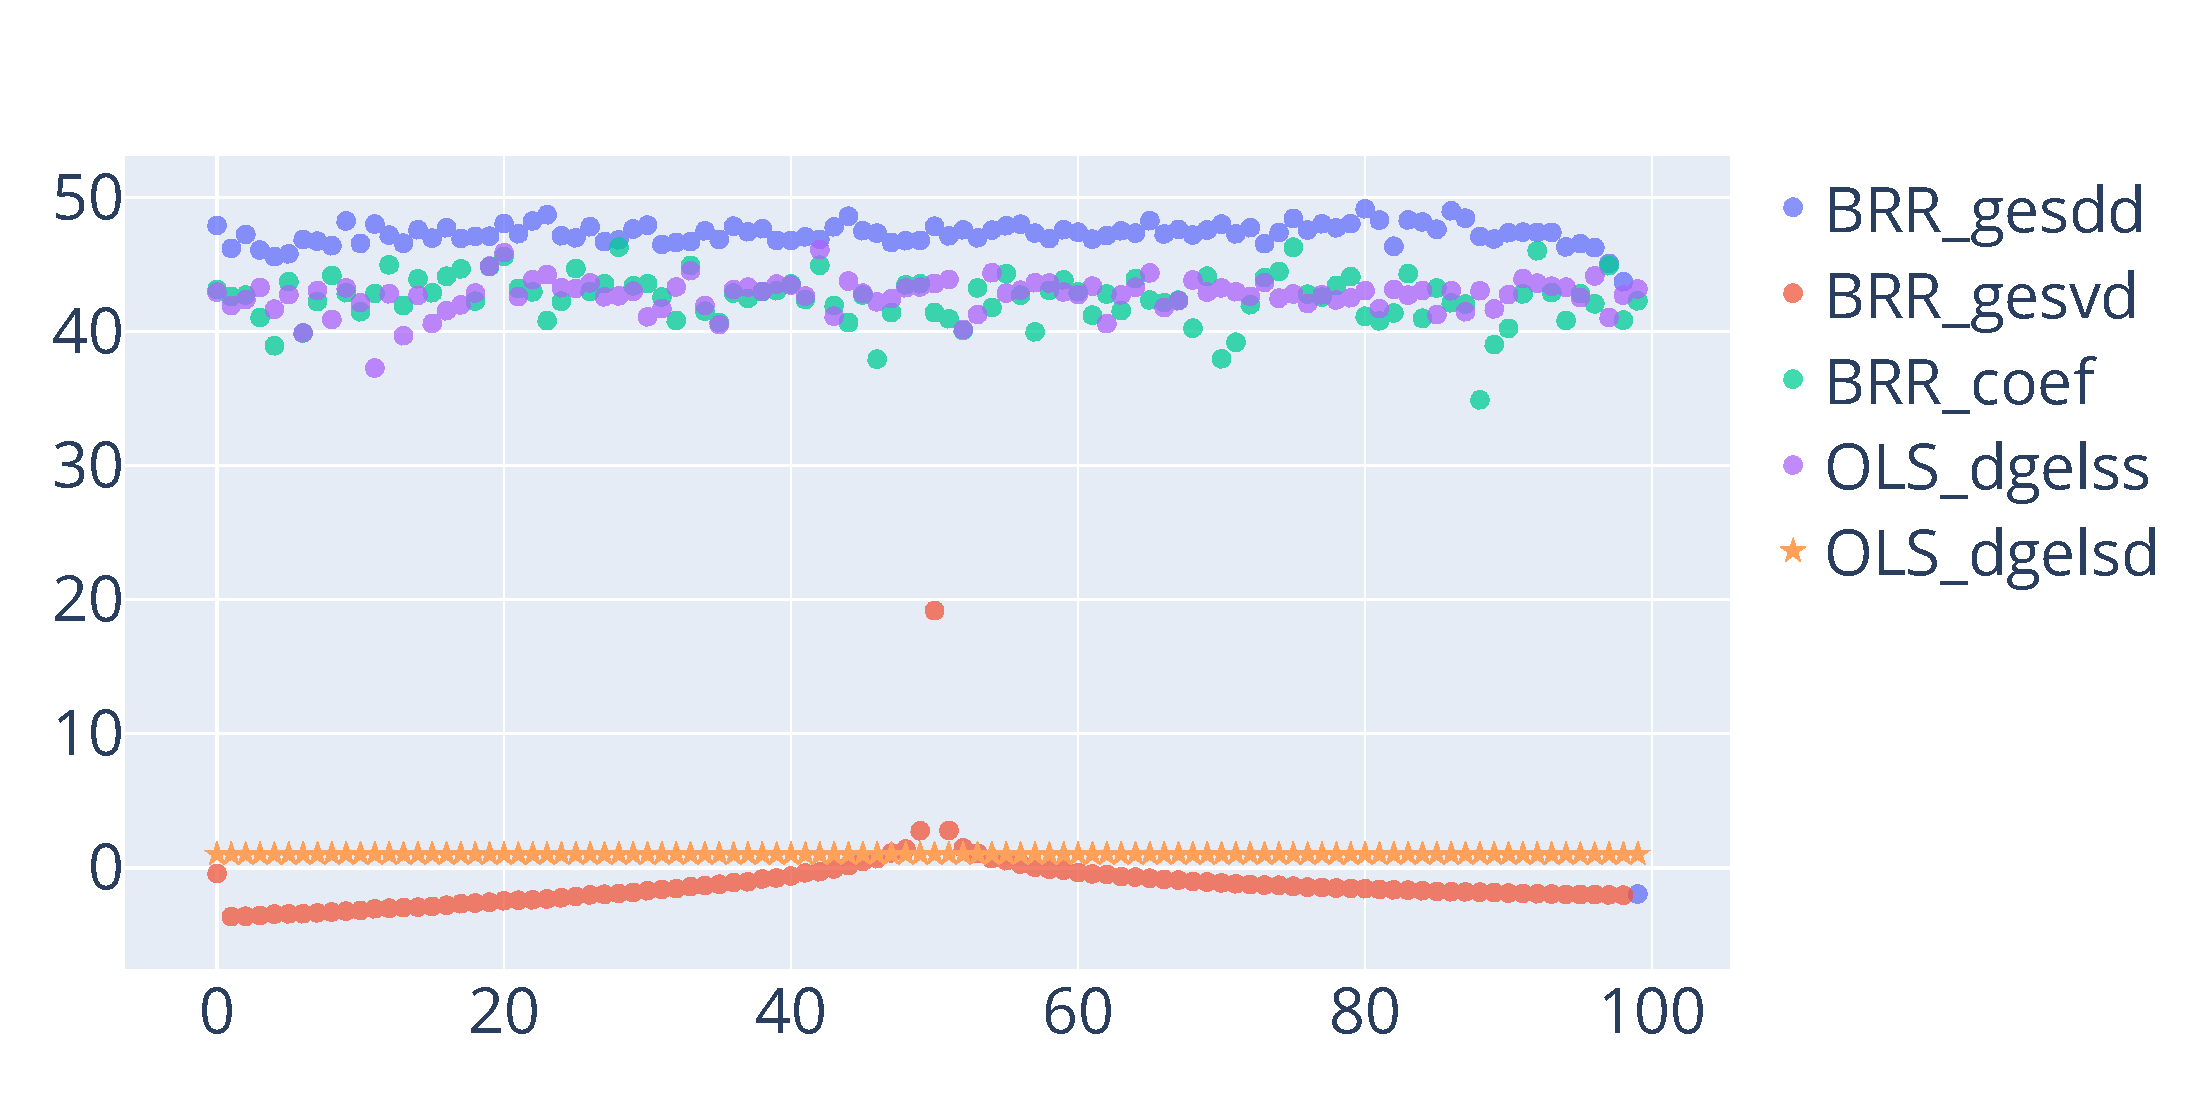
\includegraphics[width=\linewidth]{figure/BRR/BRR_coefs_sig.pdf}
%     \caption{Precision of Bayesian Ridge Regression coefficients in RR mode.
%         \texttt{BRR\_*} show the \texttt{BayesianRidge} results using the
%         \texttt{gesdd} and \texttt{gesvd} methods. \texttt{OLS\_*} show the
%         \texttt{LinearRegression} results with the \texttt{dgelsd} and
%         \texttt{dgelss} methods. The Divide \& Conquer method (\texttt{gesdd}
%         and  \texttt{dgelsd}) has low precision for \textit{BRR} and results in
%         \texttt{NaN} values (star points) for \textit{OLS}. By switching to the
%         \texttt{gesvd} method, results have a precision of 42 bits on average. }
%     \label{fig:brr_svd_sig}
% \end{figure}

% This example compares a Bayesian Ridge Regression (BRR) to the Ordinary Least
% Squares (OLS) estimator on a synthetic dataset and for one-dimensional
% regression using polynomial feature expansion. Although the example does not
% raise a runtime error, the regression coefficients computed from the fitting are
% non-significant. \pytracer traces reveal that the SVD solver used is the root
% cause for this error. Figure~\ref{fig:call_path_brr} shows the two call paths
% for BRR and OLS. The LAPACK library has two main methods for computing the SVD:
% \texttt{gesdd} and \texttt{gesvd}. The former uses a Divide \& Conquer approach,
% while the latter uses a QR decomposition. While both methods are expected to
% have the same accuracy~\cite{nakatsukasa2013stable},
% Figure~\ref{fig:brr_svd_sig} shows that \texttt{gesdd} is totally imprecise,
% with an average number of significant digits of 0\footnote{Following
%     Equation~\ref*{eq:sig-digits}, a number of significant digits below 0 means that
%     the variability ($\sigma$) is higher than the avarage value ($\mu$).} for BRR
% and even \texttt{Not-a-Number} (\texttt{NaN}) values for OLS. On the same
% figure, we can see that using the \texttt{gesvd} (\remove{dgelsd} \add{dgelss})
% method instead of the \texttt{gesdd} (\remove{dgelss} \add{dgelsd}) one, the SVD
% converges for RR and Full MCA, with a number of significant bits of 44 on
% average. This observation supports the on-going discussion among LAPACK
% developers on the instability of \texttt{gesdd} (see
% \href{https://github.com/Reference-LAPACK/lapack/issues/316}{github.com/Reference-LAPACK/lapack/issues/316}).
